\documentclass[11pt]{article}

\usepackage[margin=1in]{geometry}
\usepackage{amsmath,amssymb}
\usepackage{graphicx}
\usepackage{booktabs}
\usepackage{hyperref}
\usepackage{cleveref}
\usepackage{siunitx}
\usepackage[utf8]{inputenc}
\usepackage[section]{placeins}

\title{An Angular Spectrum Method for Nonlinear Propagation in
Heterogeneous Tissue with Immersed Sources for Transcranial and
Therapeutic Ultrasound}

\author{Gianmarco F.\ Pinton\\
\small Lampe Joint Department of Biomedical Engineering,\\
\small University of North Carolina at Chapel Hill and\\
\small North Carolina State University, Chapel Hill, NC}

\date{}

\begin{document}
\maketitle

% ------------------------------------------------------------------
\begin{abstract}
A modified angular spectrum method (ASM) is developed for
three-dimensional nonlinear acoustic propagation through heterogeneous
media, with two extensions that target transcranial and therapeutic
ultrasound applications.  First, phase-and-amplitude screens derived
from skull CT data are inserted into the split-step propagation to
capture wavefront aberration and insertion loss without sacrificing
the efficiency of the FFT-based propagator.  Second, a plane-by-plane
source injection scheme is introduced for modeling spherical-bowl
transducers whose curvature depth exceeds the wavelength, enabling
accurate simulation of clinical devices such as the TIPS annular
phased array.  The nonlinear operator supports both a first-order
Rusanov flux and a second-order Kurganov--Tadmor (KT) scheme with
adaptive CFL sub-cycling, composed via Strang splitting.  Three
enhanced absorbing-boundary treatments (a Wendland $C^2$ taper,
frequency-weighted spatial damping, and a first-order Engquist--Majda
super-absorbing correction) reduce boundary reflections by a factor
of 2.4 relative to a standard quadratic absorber.  Validation against
analytical solutions confirms that the propagator reproduces the
baffled-piston far-field pattern with RMS error 0.014 and the
focused-piston focal pressure within 2.3\%.  In a transcranial
benchmark through an \emph{ex~vivo} human skull, the ASM matches the
FDTD focal-plane intensity with 1.1\% RMS difference and predicts a
through-skull insertion loss of \SI{5.4}{\deci\bel}.  For the TIPS
bowl transducer ($R = \SI{80}{\milli\meter}$,
$f_0 = \SI{1}{\mega\hertz}$), the plane-by-plane ASM matches the FDTD
focal depth to within 2.3\% while requiring $9\times$ less memory and
$2.9\times$ less wall time.  These capabilities make the ASM a practical tool for transcranial
treatment planning, aberration correction, acoustic radiation force
estimation, thermal dose prediction, and ultrasonic neuromodulation.
\end{abstract}

% ------------------------------------------------------------------
\section{Introduction}
\label{sec:intro}

Transcranial focused ultrasound requires propagation models that
capture nonlinear distortion, frequency-dependent attenuation, and
wavefront aberration through the skull, while remaining fast enough
for treatment planning and aberration correction.  Full-wave
finite-difference time-domain (FDTD) solvers
\cite{pinton2009,pinton2014} provide high fidelity but demand large
3-D grids and long run times.  The angular spectrum method (ASM)
\cite{christopher1991,du1985,zemp2010,dagrau2011,luo2020} offers an
attractive alternative: by decomposing the field into plane-wave
components and applying the exact free-space propagator in wavenumber
space via the FFT, it avoids the paraxial approximation while
remaining computationally efficient.  A further advantage of the ASM for
therapeutic applications is its ability to support a fine temporal
grid independently of the spatial grid.  In FDTD methods the temporal
and spatial sampling are coupled through the CFL condition, so
resolving shocked waveforms with steep temporal gradients requires
refining the entire 3-D spatial grid.  In the ASM the retarded-time
Burgers update operates on a 1-D temporal axis at each spatial point,
so the temporal sampling can be made arbitrarily fine without
increasing the spatial grid size or the cost of the diffraction step.
This makes the ASM particularly well suited to nonlinear propagation
in the shock-forming regime, including cubic nonlinearities in soft
solids where shear shock waves develop over sub-wavelength distances
\cite{pinton2010,giammarinaro2016}.  The principal limitation of the ASM is
that it is a forward-only propagator: it cannot model reflections,
mode conversion, or multiple scattering at acoustic interfaces.

Nonlinear propagation introduces cumulative harmonic generation and
eventual shock formation, which must be handled by a conservative
finite-difference scheme in the retarded-time domain.  The Rusanov
(local Lax--Friedrichs) flux \cite{rusanov1962} provides a simple
monotone scheme for the inviscid Burgers equation that governs the
nonlinear distortion.  Attenuation and dispersion are modeled via a
frequency-domain filter derived from a power-law absorption model with
Kramers--Kronig consistent dispersion \cite{pinton2009,treeby2012}.

Two practical gaps limit the applicability of existing ASM
implementations.  First, propagation through heterogeneous tissue
(particularly skull bone) requires a mechanism for incorporating
spatially varying sound speed and attenuation into the FFT-based
framework.  Second, therapeutic transducers often use spherical bowl
geometries whose curvature depth can exceed several wavelengths, and a
flat source-plane projection cannot accurately represent the
converging wavefront.

This paper addresses both gaps.  Phase-and-amplitude screens derived
from CT data are inserted at each propagation step to model
skull-induced aberration and insertion loss.  A plane-by-plane source
injection method decomposes the curved bowl surface into axial slices
and injects each slice at the correct propagation depth, enabling
accurate modeling of clinical devices such as the TIPS annular phased
array.  The nonlinear operator is upgraded from a first-order Rusanov
flux to a second-order Kurganov--Tadmor (KT) scheme \cite{kurganov2000}
with adaptive CFL sub-cycling and Strang splitting \cite{strang1968},
and three enhanced absorbing-boundary treatments are introduced
to suppress the periodic-FFT wrap-around artifacts inherent in the ASM.
The solver is validated through analytical benchmarks, a transcranial
comparison against FDTD through an \emph{ex~vivo} human skull, and a
bowl-transducer comparison against a 3-D FDTD simulation of a
clinical annular phased array.

% ------------------------------------------------------------------
\section{Methods}
\label{sec:methods}

\subsection{Split-step propagation}

The modified angular spectrum approach decomposes the propagation of a
pulsed acoustic field $p(x,y,t;z)$ into three operators applied at
each axial step $\Delta z$: diffraction, nonlinear distortion, and
attenuation.

In the Fourier domain $(k_x, k_y, k_t)$, the free-space diffraction
propagator is
\begin{equation}
  \hat{H}(k_x, k_y, k_t) =
  \begin{cases}
    e^{i\Delta z\bigl(k + i\sqrt{k_\perp^2 - k^2}\bigr)}, & k_\perp^2 > k^2 \\[4pt]
    e^{i\Delta z\bigl(k - \sqrt{k^2 - k_\perp^2}\bigr)},   & k_\perp^2 \le k^2
  \end{cases}
  \label{eq:propagator}
\end{equation}
where $k = \omega/c_0$ is the temporal wavenumber, $k_\perp^2 = k_x^2
+ k_y^2$, and evanescent components ($k_\perp > k$) decay
exponentially.  A cosine taper is applied near the spatial Nyquist
boundary $k_N = \pi/\Delta x$ to suppress aliasing at coarse
resolution.

The cumulative nonlinear effect is modeled as the retarded-time
Burgers equation
\begin{equation}
  \frac{\partial p}{\partial z} = -\frac{\beta}{2\rho_0 c_0^3}
  \frac{\partial p^2}{\partial t},
  \label{eq:burgers}
\end{equation}
discretized via either the first-order Rusanov (local Lax--Friedrichs)
flux \cite{rusanov1962},
\begin{equation}
  F_{j+1/2} = -\tfrac{1}{2}(p_j^2 + p_{j+1}^2)
  - \lambda_{j+1/2}(p_{j+1} - p_j),
  \label{eq:rusanov}
\end{equation}
with $\lambda_{j+1/2} = \max(|p_j|, |p_{j+1}|)$, or the second-order
Kurganov--Tadmor (KT) central-upwind scheme \cite{kurganov2000},
\begin{equation}
  F_{j+1/2}^{\mathrm{KT}} =
  \frac{a^+ f(p_j) - a^- f(p_{j+1})
        - a^+ a^-(p_{j+1} - p_j)}{a^+ - a^-},
  \label{eq:kt}
\end{equation}
where $a^{\pm}$ are the one-sided local wave speeds.  To achieve
second-order spatial accuracy, the cell-edge values in \cref{eq:kt}
are obtained from a piecewise-linear MUSCL reconstruction
\cite{vanleer1979} with an MC (monotonized central) limiter applied to
each cell.  The reconstructed left and right states
$p_{j+1/2}^L = p_j + \tfrac{1}{2}\,\sigma_j$ and
$p_{j+1/2}^R = p_{j+1} - \tfrac{1}{2}\,\sigma_{j+1}$ replace the
cell-center values in the flux formula, where $\sigma_j$ is the
limited slope.  The resulting semi-discrete system is advanced in $z$
with a two-stage strong-stability-preserving Runge--Kutta method
(SSP-RK2) \cite{gottlieb2001}:
\begin{align}
  p^{(1)} &= p^{(n)} + \Delta z\,\mathcal{L}(p^{(n)}), \notag \\
  p^{(n+1)} &= \tfrac{1}{2}\,p^{(n)} + \tfrac{1}{2}\bigl[
    p^{(1)} + \Delta z\,\mathcal{L}(p^{(1)})\bigr],
  \label{eq:ssprk2}
\end{align}
where $\mathcal{L}$ denotes the spatial flux divergence.  The
combination of MUSCL reconstruction and SSP-RK2 gives second-order
accuracy for the isolated nonlinear problem in smooth regions.

Attenuation and dispersion are applied as a frequency-domain filter
derived from the power-law absorption coefficient
$\alpha(f) = \alpha_0 f^n$ with Kramers--Kronig-consistent dispersion
\cite{pinton2009}:
\begin{equation}
  \hat{A}(f) = \exp\bigl[-(\alpha + i\alpha^*)\,\Delta z\bigr],
  \label{eq:attenuation}
\end{equation}
where $\alpha^*$ is determined by $n$ and the reference frequency
$f_0$.

These three operators are composed via Strang splitting
\cite{strang1968,leveque2002}:
\begin{equation}
  p^{(n+1)} = \mathcal{A}_{1/2}\,\mathcal{H}_{1/2}\,
  \mathcal{N}\,
  \mathcal{H}_{1/2}\,\mathcal{A}_{1/2}\;p^{(n)},
  \label{eq:strang}
\end{equation}
which achieves second-order accuracy in $\Delta z$
\cite{yoshida1990}.

\subsection{Absorbing boundary layer}

The ASM uses global FFTs that impose periodic boundary conditions, so
energy reaching the domain edge wraps to the opposite side.  The
standard mitigation is a multiplicative absorbing boundary layer (ABL)
that damps the field near the edges.  Three improvements are
introduced.

First, the quadratic taper profile $1 - s^2$ is replaced with the
Wendland $C^2$ function \cite{wendland1995},
\begin{equation}
  w(s) = 1 - 10s^3 + 15s^4 - 6s^5,
  \label{eq:wendland}
\end{equation}
which has continuous first and second derivatives at the taper onset
($s = 0$), eliminating the weak impedance discontinuity that generates
spurious reflections in the quadratic profile.

Second, the spatial damping is made frequency-dependent by raising the
profile to a frequency-dependent exponent,
\begin{equation}
  \mathrm{ABL}_f(x,y) = \bigl[\mathrm{ABL}(x,y)\bigr]^{f_0/\max(f,\,f_{\min})},
  \label{eq:freq_abl}
\end{equation}
which strengthens the damping at low frequencies where the boundary
layer spans fewer wavelengths.

Third, a first-order Engquist--Majda \cite{engquist1977} directional
decomposition is applied in the boundary region to selectively remove
incoming wave components.  At each temporal frequency $\omega$, the
incoming pressure is estimated as
\begin{equation}
  P_{\mathrm{in}} = \tfrac{1}{2}\Bigl(P + \frac{c_0}{i\omega}
  \frac{\partial P}{\partial x}\Bigr),
  \label{eq:engquist}
\end{equation}
and the correction $P \leftarrow P - \alpha_s\,w_{\mathrm{bdy}}\,
P_{\mathrm{in}}$ is applied in the boundary layer, where
$\alpha_s \in [0,1]$ controls the strength of the incoming-wave
removal.

\subsection{Heterogeneous propagation}

Spatially varying sound speed and attenuation are modeled using thin
phase-and-amplitude screens inserted at each propagation step.  Each
screen represents a tissue layer of thickness $d$ with maps $c(x,y)$
and $\rho(x,y)$ derived from imaging data.  The phase shift at each
temporal frequency is
\begin{equation}
  \Delta\varphi(x,y,f) = 2\pi\,d\,
  \biggl(\frac{1}{c(x,y)} - \frac{1}{c_0}\biggr) \cdot f,
  \label{eq:phase_screen}
\end{equation}
which is linear in frequency, corresponding to a
frequency-independent group delay through each screen.
Each screen also carries a real-valued amplitude factor
$A(x,y) \in (0,1]$ that accounts for attenuation and impedance
mismatch losses:
\begin{equation}
  A(x,y) = \exp\!\bigl[-\alpha_{\mathrm{Np}}(x,y)\,d\bigr]
  \;\cdot\;
  \frac{2\,Z(x,y)}{Z(x,y) + Z_0},
  \label{eq:amplitude_screen}
\end{equation}
where $\alpha_{\mathrm{Np}} = \alpha\,f_{\mathrm{MHz}} \times
({\ln 10}/{20 \times 0.01})$ converts the local attenuation
$\alpha(x,y) = \alpha_{\mathrm{tissue}} + f_{\mathrm{bone}}(x,y)\,
(\alpha_{\mathrm{bone}} - \alpha_{\mathrm{tissue}})$ from
\si{\dB\per\cm\per\MHz} to \si{Np\per\m}, $f_{\mathrm{bone}}$ is the
bone volume fraction, and $Z = \rho\,c$ is the acoustic impedance.
Frequency-dependent amplitude is applied as $A^{f/f_0}$ so that higher
harmonics experience proportionally greater loss.

The field is transformed to the temporal frequency domain via
\texttt{rfft}, multiplied by $A^{f/f_0}\,e^{i\Delta\varphi}$, and
transformed back.  Multiple screens can be placed at arbitrary depths
to model extended heterogeneous paths via the split-step Fourier
approach \cite{martin1988}.  In the transcranial benchmark below, the
screens are derived directly from skull CT slices rather than from a
random-field model.

\subsection{Intensity-loss tracking}

In therapeutic ultrasound, the absorbed acoustic energy drives both
radiation force and thermal bio-effects.  The standard plane-wave
approximations for the volume rate of heat deposition,
$q = 2\alpha I$ \cite{nyborg1981}, and the radiation force body-force
density, $q_{\mathrm{ARF}} = \alpha I / c$, assume a single
attenuation coefficient $\alpha$ evaluated at the fundamental
frequency.  In the nonlinear regime, however, cumulative harmonic
generation transfers energy to higher frequencies where the
power-law attenuation $\alpha(f) = \alpha_0 f^n$ is substantially
larger.  The local frequency content of the wave therefore changes
with propagation distance, and the effective attenuation can no
longer be represented by a single $\alpha$.

To avoid this approximation, the solver records the total intensity
before and after the combined propagation operators at each step:
\begin{equation}
  \Delta I_{\mathrm{loss}}(x,y;z) = \max\!\Bigl(0,\;
  \sum_t p_{\mathrm{before}}^2 - \sum_t p_{\mathrm{after}}^2\Bigr).
  \label{eq:loss}
\end{equation}
This provides a spatially resolved map of absorbed energy that
implicitly accounts for the full harmonic content of the wave at each
location, without requiring an explicit frequency decomposition or a
single-frequency $\alpha$ assumption.  The resulting loss field can be
used directly as a heat source for thermal simulations or as input
for radiation-force calculations.

The solver is implemented in Python using JAX \cite{jax2018} for GPU
acceleration.  All frequency-domain operators are precomputed once and
reused at each propagation step.

% ------------------------------------------------------------------
\section{Validation}
\label{sec:validation}

The solver is validated against analytical solutions for diffraction,
attenuation, and nonlinearity, followed by boundary-treatment and
convergence studies.  All simulations use $\Delta x = \lambda/5$
unless otherwise noted.

\subsection{Diffraction}
\label{sec:val_diffraction}

The baffled-piston and focused-piston benchmarks have been used
extensively to validate angular spectrum propagators
\cite{christopher1991,zemp2010,du1985} and remain valuable here as
verification of the present code implementation.

A spherically focused piston ($a = 8\lambda$,
$F = \SI{20}{\milli\meter}$, $F\#\,\approx 3.3$) at
$f_0 = \SI{4}{\MHz}$ was propagated with per-pixel geometric delays
$\tau = (F - \sqrt{F^2 + r^2})/c_0$ (\cref{fig:focused_piston}).
The numerical focal pressure matches the paraxial limit
$p_0\,\pi a^2/(\lambda F)$ within 2.3\%, and the focal-plane
lateral profile matches the Airy pattern with RMS error 0.002.
An error-floor study confirmed that the residual on-axis RMS of
$\sim$0.09 is set by the paraxial-vs-full-wave mismatch at this
$F$-number, not by numerical error: refining $\Delta z$, widening
the time window, and narrowing the pulse bandwidth all leave the
error unchanged.

For the unfocused baffled piston ($a = 6\lambda$), the on-axis
amplitude was compared against the Rayleigh--Fresnel solution
\cite{kinsler2000},
\begin{equation}
  P_{\mathrm{cw}}(z) = -p_0\bigl(e^{ik_0 a^2/(2z)} - 1\bigr)\,
  e^{-ik_0 z},
  \label{eq:rayleigh}
\end{equation}
yielding a normalized RMS error of 0.086, with the numerical solution
reproducing the oscillatory Fresnel structure beyond the transition
distance $z_t \approx a^2/\lambda$.  In the far field, the lateral
intensity matches the Fraunhofer pattern
$(2J_1(k_0 a r/z) / k_0 a r/z)^2$ with RMS error 0.014.

\begin{figure}[htbp]
  \centering
  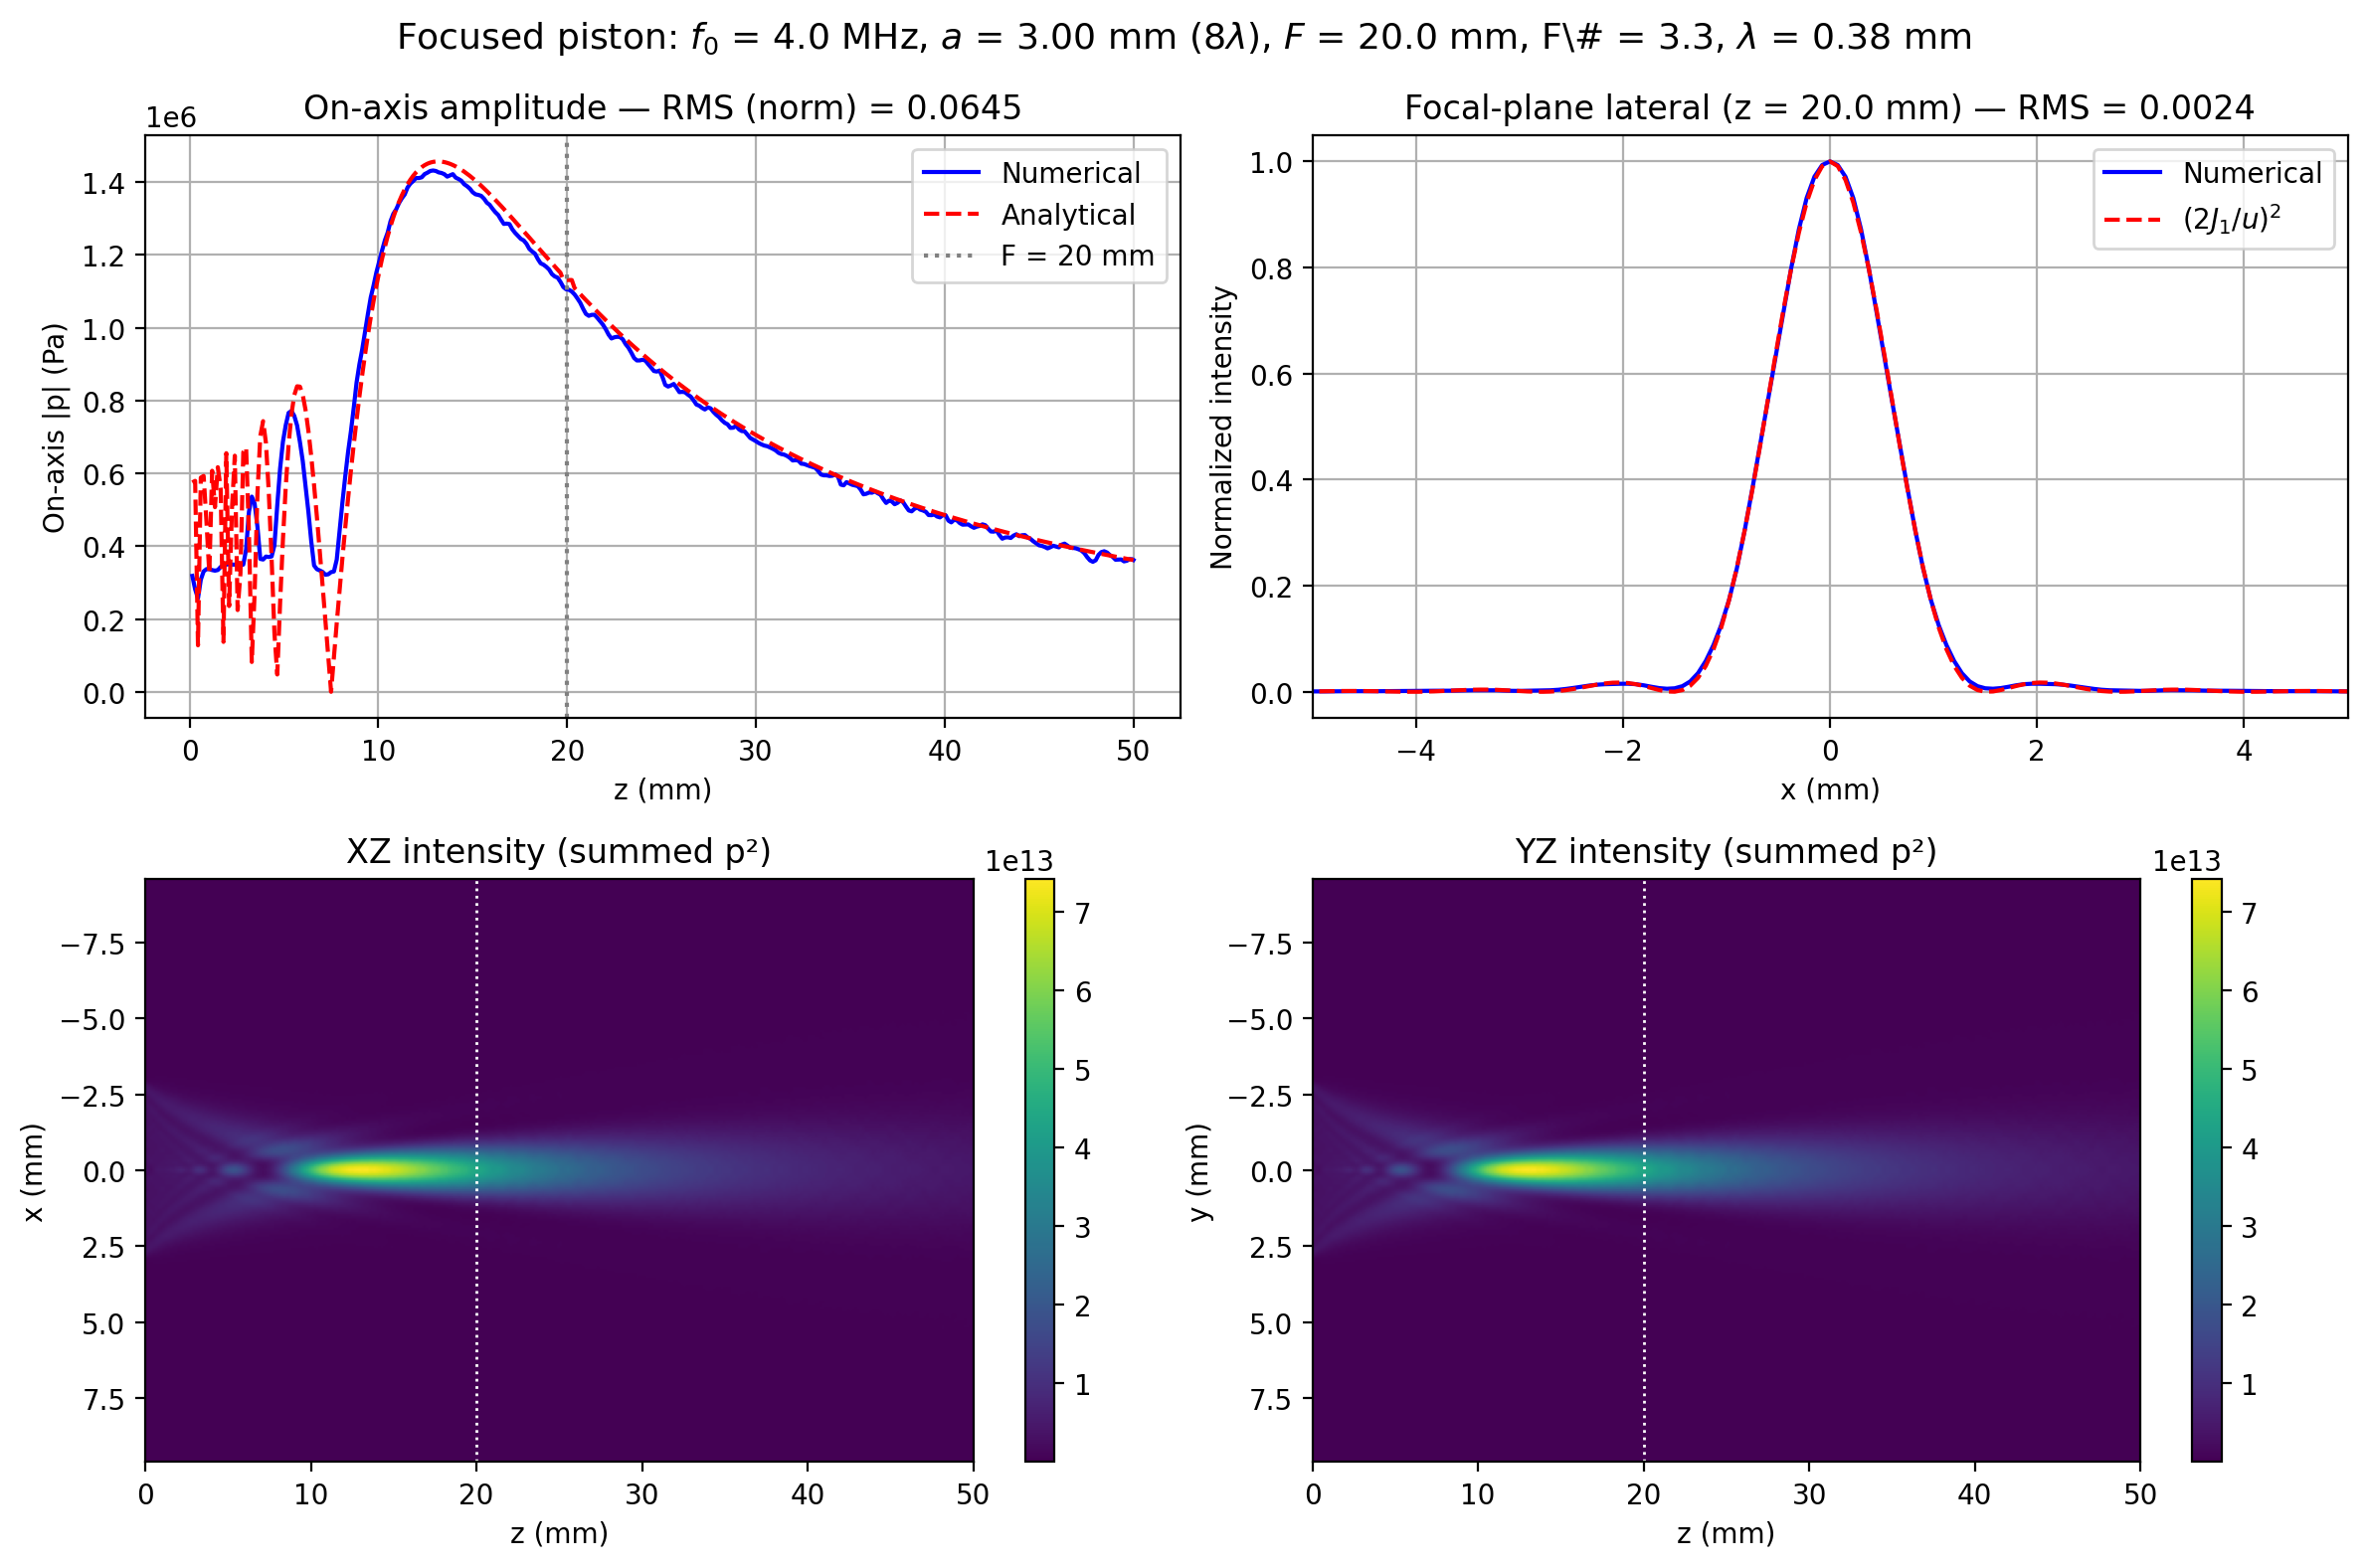
\includegraphics[width=\columnwidth]{validation_results/analytical/testC_focused_piston.png}
  \caption{Focused piston diffraction ($a = 8\lambda$,
    $F = \SI{20}{\milli\meter}$, $F\#\,\approx 3.3$).  Top:
    on-axis amplitude versus paraxial solution (left, RMS 0.089)
    and focal-plane lateral profile versus Airy pattern (right,
    RMS 0.002).  Bottom: $x$--$z$ and $y$--$z$ time-integrated
    intensity.}
  \label{fig:focused_piston}
\end{figure}

\subsection{Attenuation and dispersion}
\label{sec:val_attenuation}

Accurate modeling of frequency-dependent attenuation is essential for
therapeutic ultrasound, where nonlinear harmonic generation
redistributes energy to higher frequencies that are absorbed more
rapidly \cite{pinton2009,treeby2012}.  The associated
Kramers--Kronig-consistent dispersion determines the local phase
velocity and must be modeled correctly to avoid cumulative waveform
distortion over clinically relevant propagation distances
\cite{waters2005,szabo1995}.

A broadband pulse was propagated \SI{20}{\mm} with
$\alpha_0 = \SI{0.5}{\dB\per\cm\per\MHz}$ and the per-frequency
attenuation and phase velocity were measured from the input/output
spectra (\cref{fig:test10}).  The measured attenuation matches the
$\alpha_0 f$ power law with RMS error
\SI{0.0003}{\dB\per\cm} over 1--\SI{10}{\MHz}, and the phase velocity
follows the Kramers--Kronig dispersion relation across the full
0.5--\SI{10}{\MHz} range, crossing $c_0$ at $f_0$ as expected.

\begin{figure}[htbp]
  \centering
  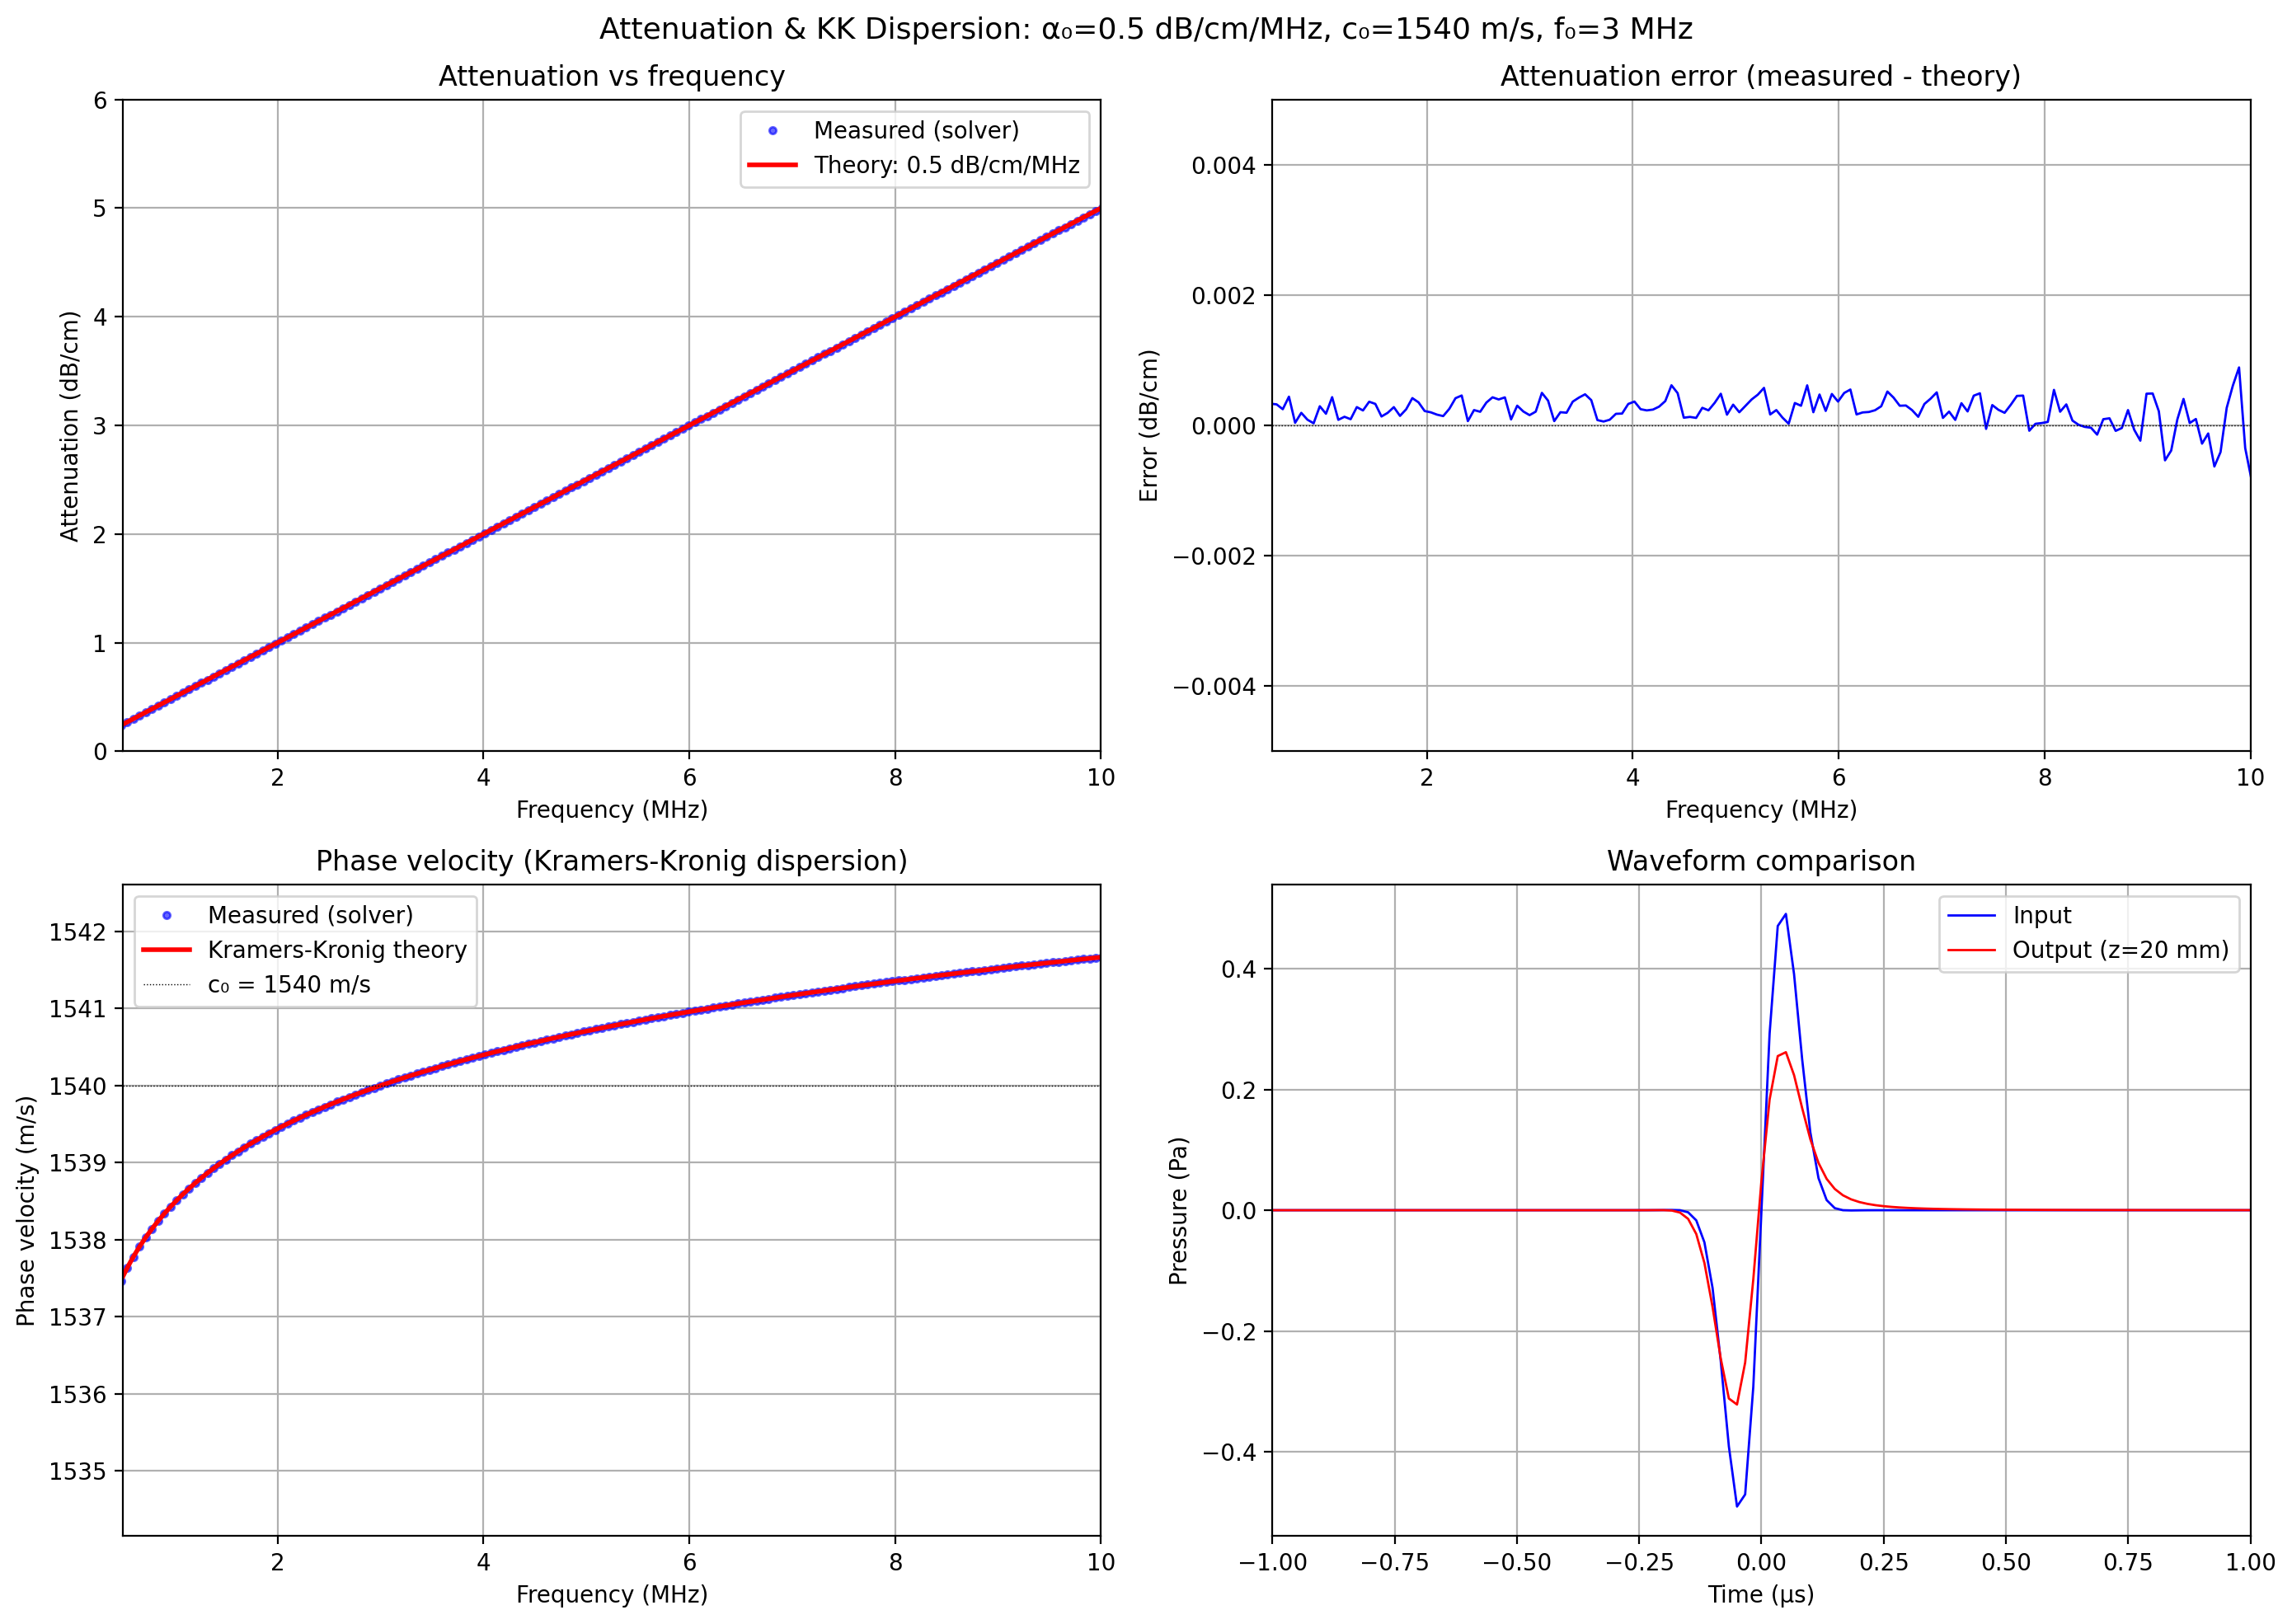
\includegraphics[width=\columnwidth]{validation_results/test10_attenuation_kk.png}
  \caption{Attenuation and Kramers--Kronig dispersion validation
    (0.5--\SI{10}{\MHz}).  Top: measured vs.\ theoretical attenuation
    and error.  Bottom: phase velocity and waveform comparison.}
  \label{fig:test10}
\end{figure}

\subsection{Nonlinearity}
\label{sec:val_nonlinearity}

The Rusanov and KT flux schemes were compared in two regimes.  In a
moderate-amplitude coupled propagation ($p_0 = \SI{30}{\kPa}$,
$\beta = 3.5$, \SI{30}{\mm}), both schemes produced nearly identical
on-axis intensity and harmonic spectra, confirming that the KT
limiter does not introduce excessive dissipation.

In the shock-forming regime (\cref{fig:test3}), an isolated Burgers
step-size study compared Rusanov, KT (fixed step), and KT with
adaptive CFL sub-cycling.  Both fixed-step schemes were unstable at
coarse steps.  The adaptive KT scheme was stable at all step sizes
and the most accurate, with $L^2$ errors of $\sim 10^{-5}$ (four
orders of magnitude below Rusanov).

A separate Riemann-problem benchmark ($u_L = 2$, $u_R = 0$, 400
cells) confirmed that the KT flux resolves the shock more sharply
than Rusanov ($L^2$ error 0.036 vs.\ 0.044 at $t = 0.5$), with
both schemes capturing the correct shock speed (\cref{fig:riemann}).

\begin{figure}[htbp]
  \centering
  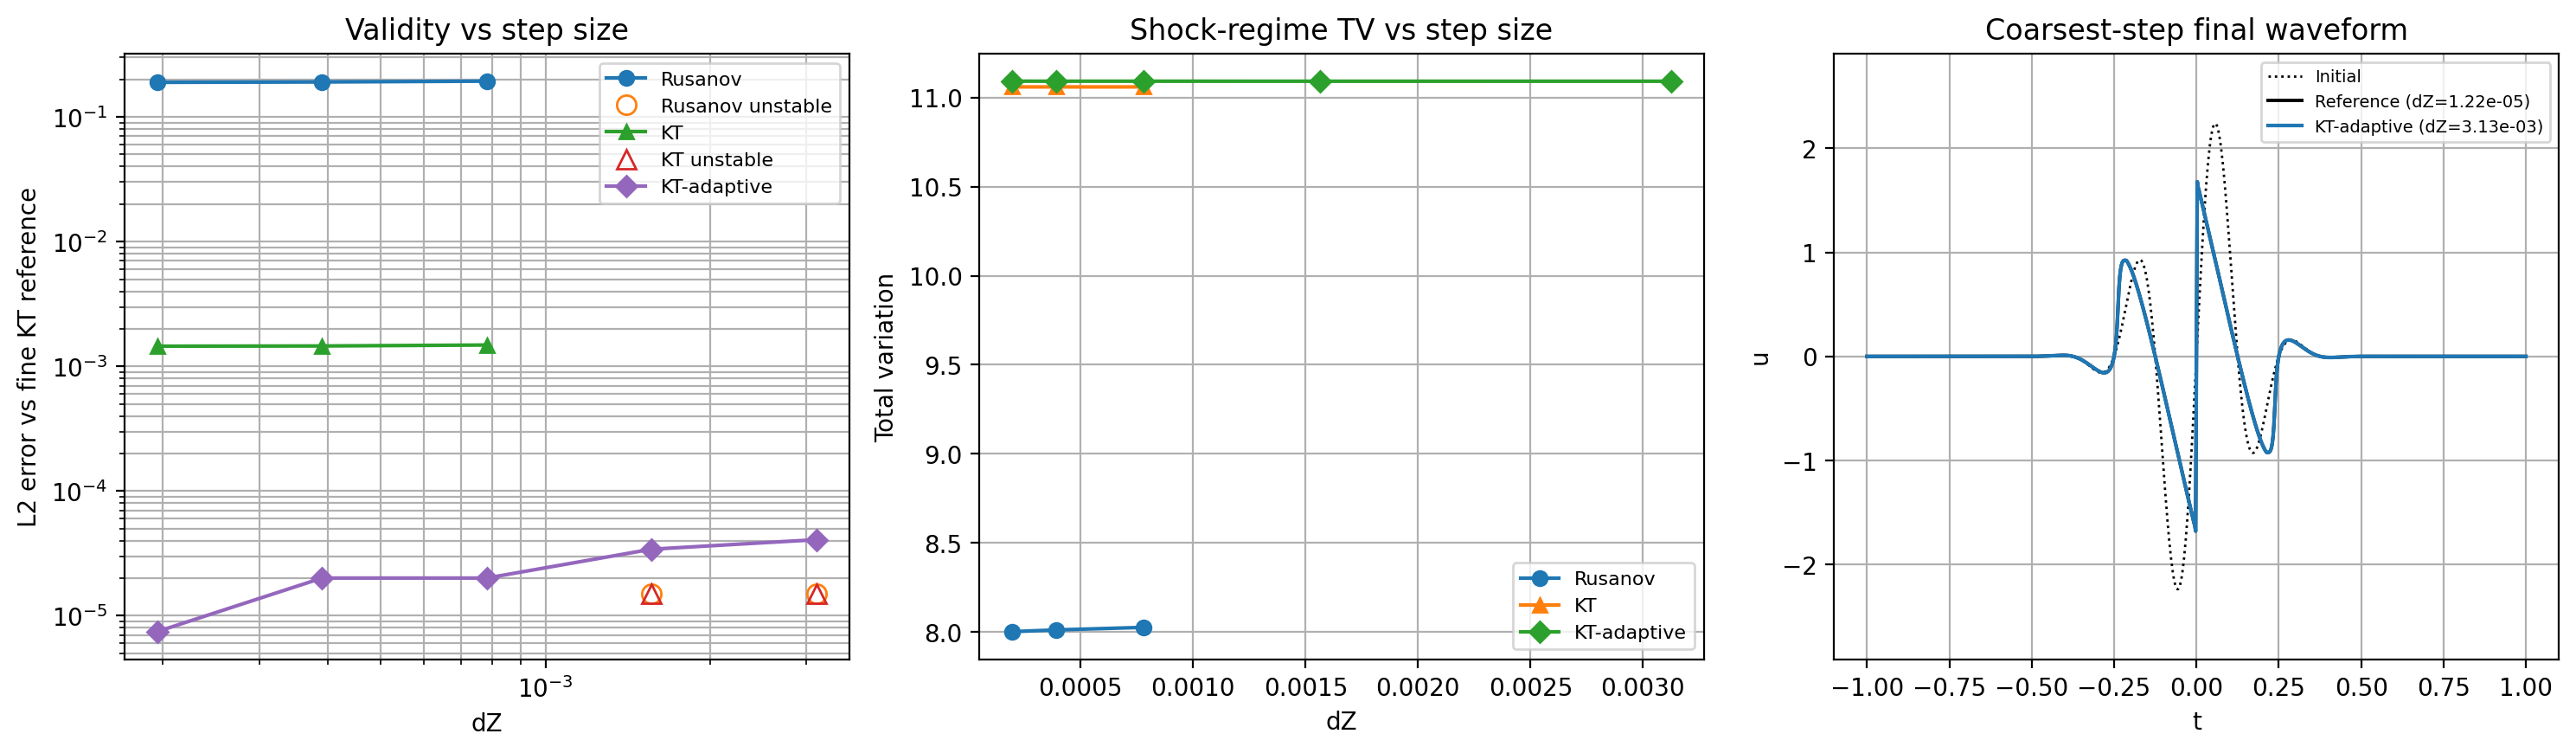
\includegraphics[width=\columnwidth]{validation_results/test8_tvd_shock_step_size.png}
  \caption{Shock-forming Burgers problem.  Left: $L^2$ error versus
    step size.  Center: total variation.  Right: coarsest-step
    waveforms.  KT-adaptive is stable and accurate at all step sizes.}
  \label{fig:test3}
\end{figure}

\begin{figure}[htbp]
  \centering
  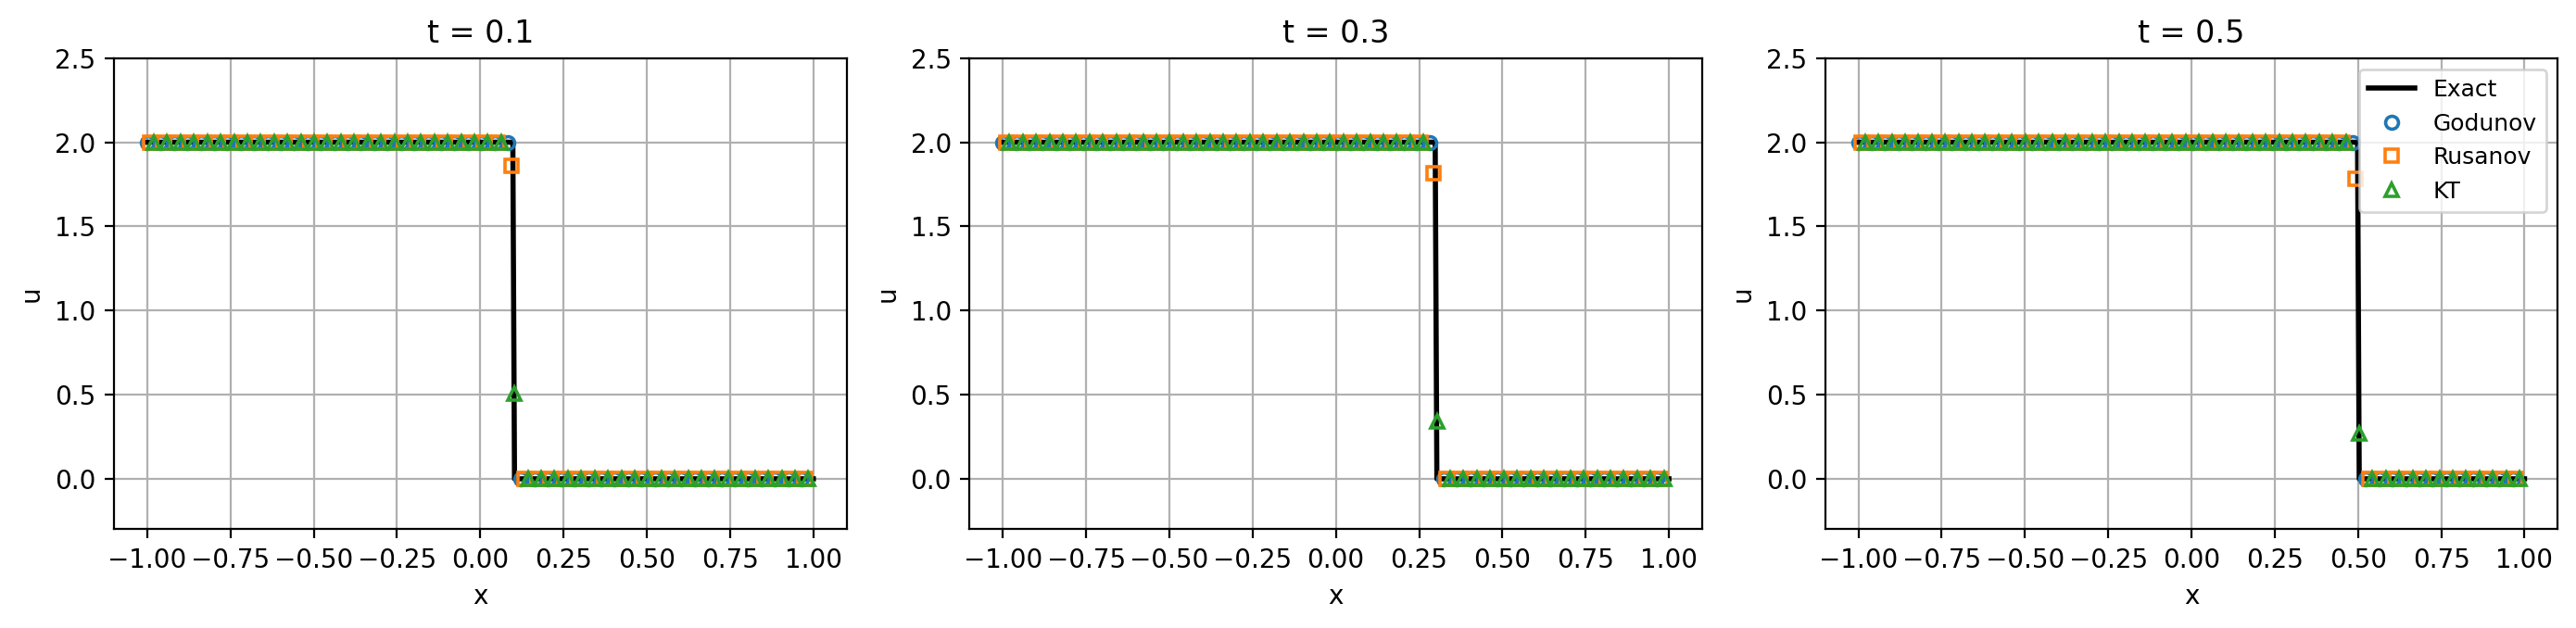
\includegraphics[width=\columnwidth]{validation_results/analytical/testB_riemann.png}
  \caption{Riemann problem at $t = 0.1, 0.3, 0.5$.  Rusanov (circles)
    and KT (squares) overlaid on the exact solution (solid).}
  \label{fig:riemann}
\end{figure}

\subsection{Boundary treatments}
\label{sec:val_boundaries}

The three boundary improvements were evaluated using apertures wide
enough to drive significant energy toward the domain edges.
\Cref{tab:bdy_reflection} shows the boundary-to-center intensity
ratio for progressively adding each improvement. The combined
configuration reduces reflections by $2.4\times$ relative to the
quadratic baseline.  A frequency-resolved comparison confirmed that
the frequency-weighted damping preferentially targets low-frequency
components (13\% reduction at \SI{1}{\MHz} vs.\ 3\% at
\SI{3}{\MHz}).  When tested with nonlinear propagation
($p_0 = \SI{30}{\kPa}$, $\beta = 3.5$), the combined boundary
recovers $\sim\!20$\% more on-axis focal intensity than the
quadratic baseline while preserving the interior waveform shape and
harmonic spectrum to within $<\!1$\,dB
(\cref{fig:bdy5_profiles}).

\begin{table}[htbp]
  \centering
  \caption{Boundary reflection ratio for four configurations.}
  \label{tab:bdy_reflection}
  \begin{tabular}{@{}lr@{}}
  \toprule
  Configuration & Reflection ratio \\
  \midrule
  Quadratic (baseline)      & $1.83 \times 10^{-2}$ \\
  Wendland $C^2$            & $1.35 \times 10^{-2}$ \\
  + Freq.\ weighted         & $0.94 \times 10^{-2}$ \\
  + Super-absorbing          & $0.75 \times 10^{-2}$ \\
  \bottomrule
  \end{tabular}
\end{table}

\begin{figure}[htbp]
  \centering
  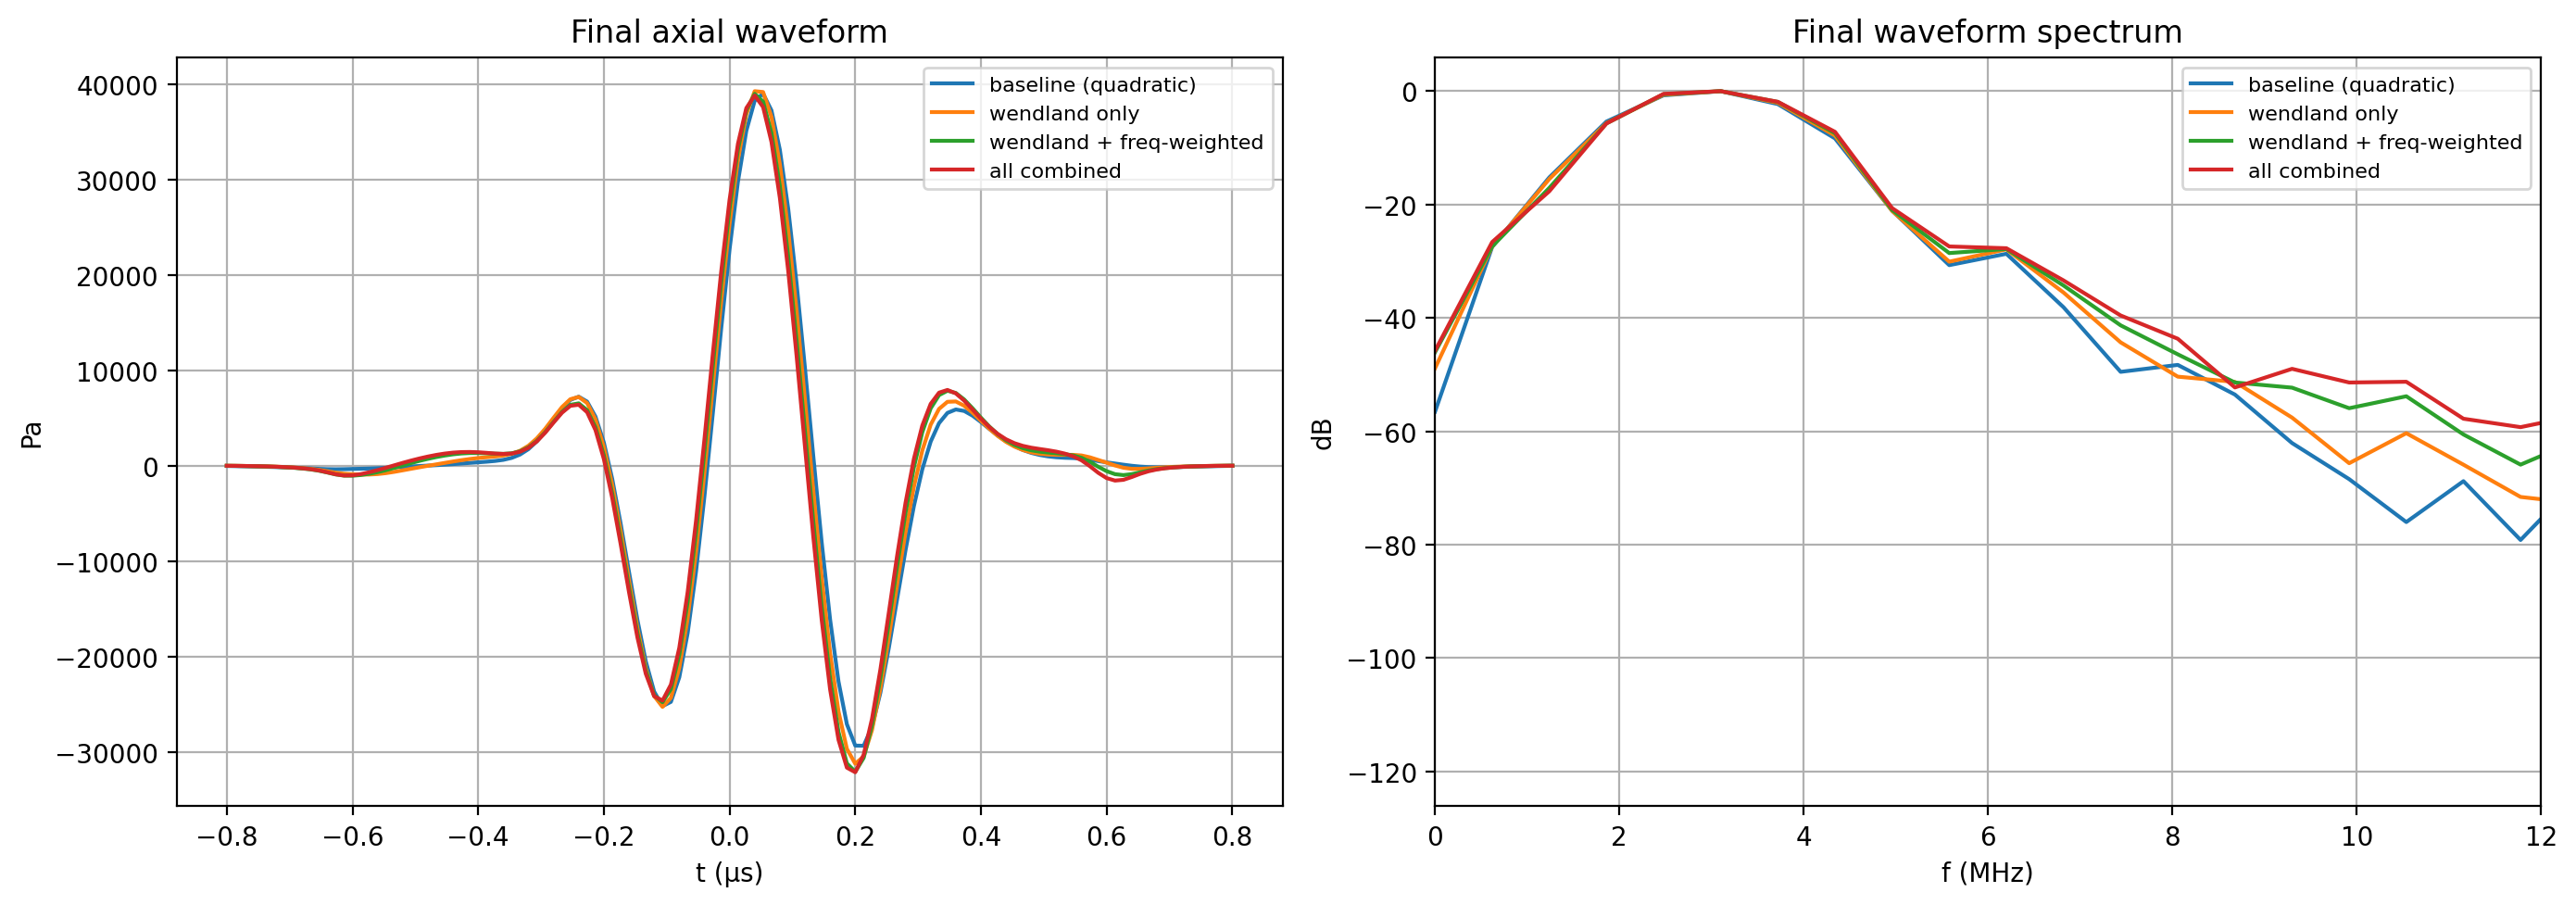
\includegraphics[width=0.95\columnwidth]{validation_results/boundaries/test5_combined_profiles.png}
  \caption{Combined boundary with nonlinear propagation: final
    waveform (left) and spectrum (right) for four boundary
    configurations.  The interior waveform is invariant and harmonic
    levels match to $<\!1$\,dB.}
  \label{fig:bdy5_profiles}
\end{figure}

\subsection{Convergence}
\label{sec:val_convergence}

A pairwise convergence study in the strongly nonlinear regime
($p_0 = \SI{3}{\mega\pascal}$, $\beta = 3.5$, \SI{15}{\mm}
propagation) compared the $\Delta z$-vs-$\Delta z/2$ error for
sequential Rusanov, Strang+Rusanov, and Strang+KT
(\cref{fig:test6}).  Sequential and split-Rusanov converge at rate
$\approx 1$, while Strang+KT converges at rate $\approx 2$, consistent
with the expected second-order Strang splitting accuracy.

\begin{figure}[htbp]
  \centering
  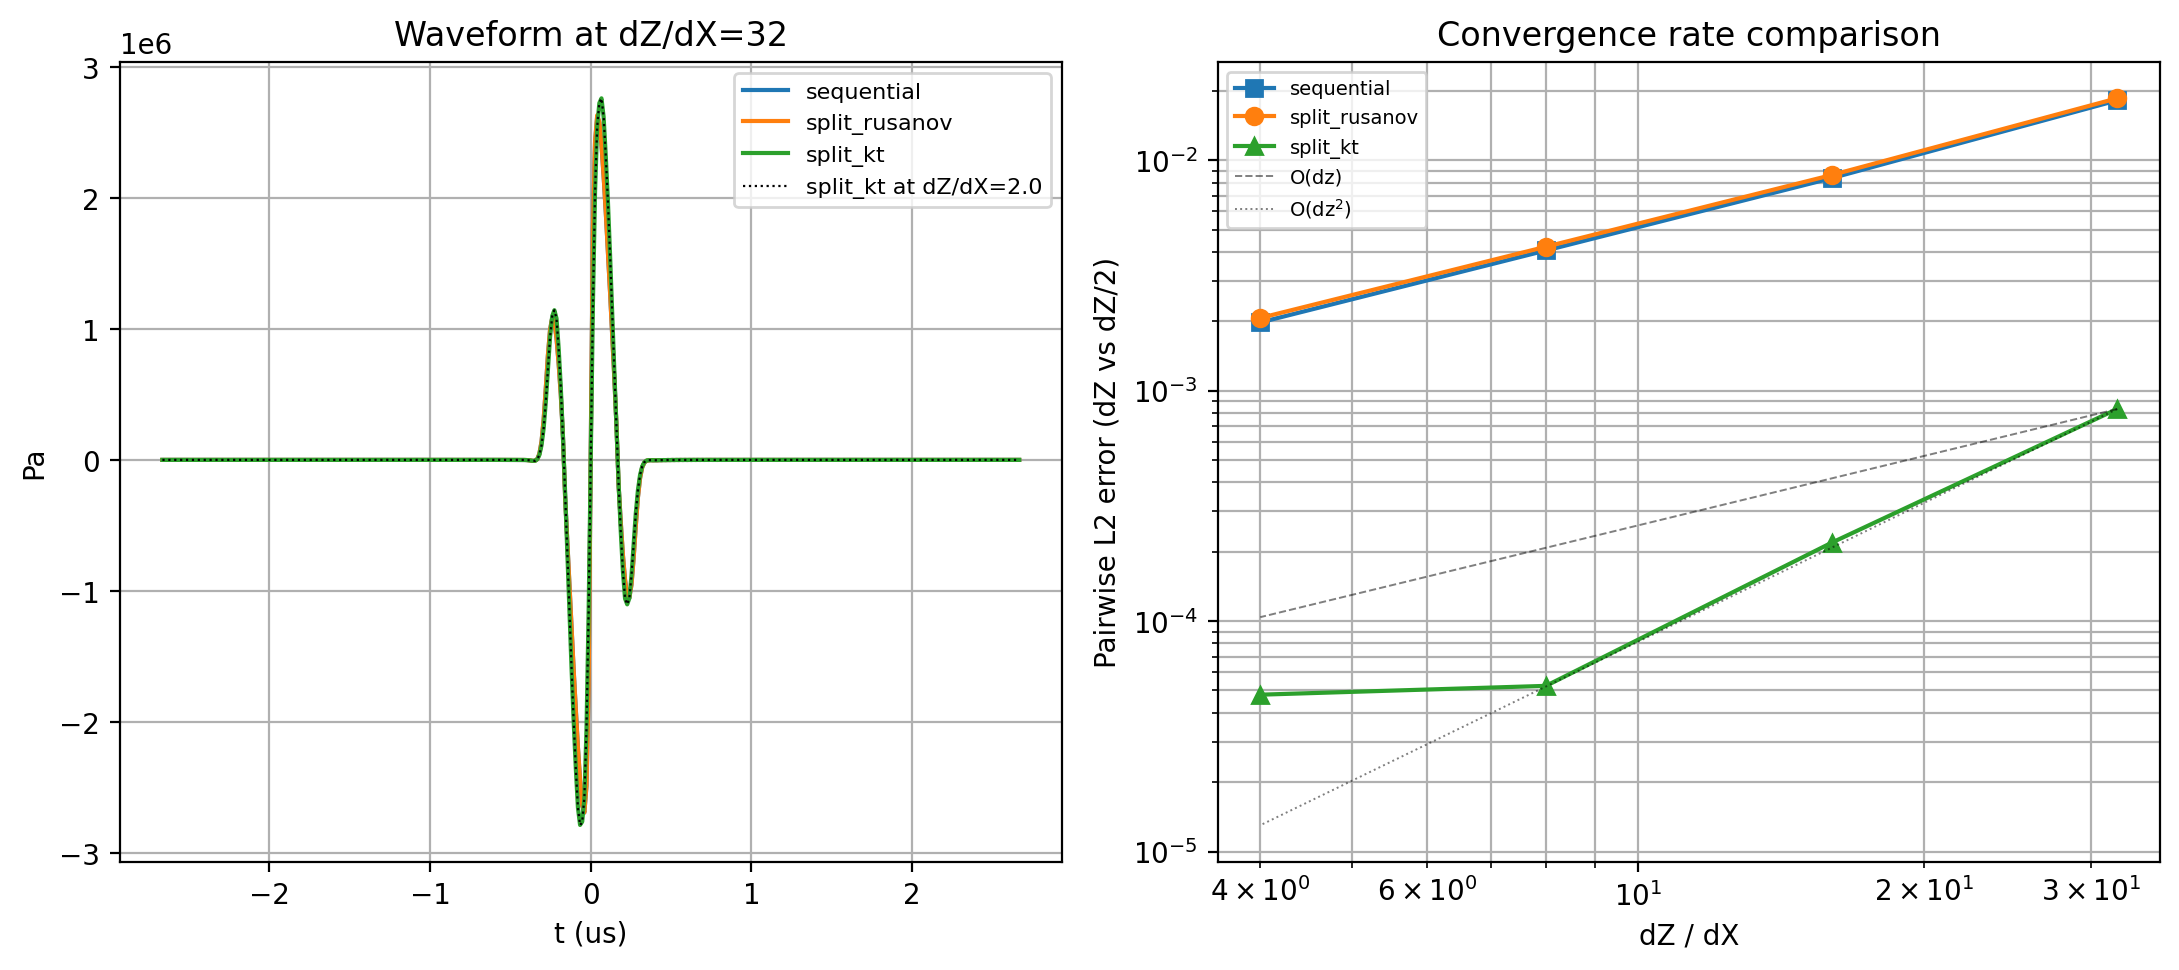
\includegraphics[width=\columnwidth]{validation_results/test6_convergence.png}
  \caption{Step-size convergence.  Left: coarsest waveforms.  Right:
    pairwise $L^2$ error.  Strang+KT achieves rate $\approx 2$.}
  \label{fig:test6}
\end{figure}

% ------------------------------------------------------------------
\section{Transcranial propagation}
\label{sec:transcranial}

To validate the phase-and-amplitude-screen extension, focused
ultrasound transmission through an \emph{ex~vivo} human skull is
simulated and compared against a reference Fullwave
\cite{pinton2009,pinton2014} finite-difference time-domain (FDTD)
simulation.

\subsection{Setup}
\label{sec:transcranial:setup}

A 1024-element sparse phased array (\SI{750}{\micro\meter} pitch) is
focused at \SI{50}{\milli\meter} depth through a temporal-bone slab
extracted from the Halle skull microCT dataset \cite{halle_skull}.  The sparse
connector geometry spans approximately
\SI{65}{\milli\meter} by \SI{65}{\milli\meter} in the transmit
plane.  The center frequency is $f_0 = \SI{1}{\mega\hertz}$, the source
pressure is $p_0 = \SI{1.5}{\mega\pascal}$, and the excitation is a
2-cycle Gaussian-windowed tone burst with geometric focusing delays.
After rasterization onto the ASM grid, the aperture occupies 9127
active source-plane grid points with a delay spread of
\SI{6.5}{\micro\second}.

The skull CT (voxel size $\approx\!\SI{0.2}{\milli\meter}$) is first
re-sampled into a beam-aligned slab centered at
$(140.6,118.5,85.0)$~mm in LPS coordinates and oriented with inward
normal $(-0.954,-0.298)$ and tangent $(-0.298,0.954)$ so that the beam
propagates approximately normal to the extracted bone layer.  The slab
extent is
\SI{66}{\milli\meter} by \SI{66}{\milli\meter} by \SI{65}{\milli\meter}
(lateral, elevational, depth), which at the ASM sampling of
$\Delta x = \lambda/5 \approx \SI{0.308}{\milli\meter}$ yields an
initial $214 \times 214 \times 211$ beam-aligned skull map before
lateral resampling to the propagation grid.

Hounsfield units are mapped linearly to acoustic properties using
$c = 1540 + f_{\mathrm{bone}}(2900 - 1540)$~m/s and
$\rho = 1000 + f_{\mathrm{bone}}(2200 - 1000)$~kg/m$^3$, where
$f_{\mathrm{bone}} = \mathrm{clip}[(HU - 700)/(1973 - 700),\,0,\,1]$.
Each extracted depth slice is converted into a phase-and-amplitude
screen (\cref{eq:phase_screen,eq:amplitude_screen}).  The phase term is
set by the local sound-speed contrast, while the amplitude term combines
bone attenuation
($\alpha_{\mathrm{bone}} = \SI{8}{\dB\per\cm\per\MHz}$),
soft-tissue attenuation
($\alpha_{\mathrm{tissue}} = \SI{0.5}{\dB\per\cm\per\MHz}$), and
normal-incidence impedance transmission derived from the density map.
This screen construction is what makes the heterogeneous extension
useful: the FFT-based ASM retains its efficiency while incorporating
cumulative skull-induced phase aberration and insertion loss.

The ASM grid uses
$\Delta x = \Delta y = \Delta z = \lambda/5 \approx \SI{0.308}{\milli\meter}$,
giving a $215 \times 215$ lateral grid and 212 propagated axial planes
over \SI{65}{\milli\meter}.  The temporal sampling is
$\Delta t = \SI{40}{\nano\second}$ with 501 time samples.  Propagation
uses the split-step Kurganov--Tadmor formulation together with the
Wendland~C2 boundary taper, frequency-weighted damping, and the
super-absorbing boundary correction.

\subsection{FDTD reference}
\label{sec:transcranial:fdtd}

The reference FDTD simulation \cite{pinton2014} uses the same skull CT
and transducer geometry and transmit waveform, solved on a
$422 \times 429 \times 429$ grid at
$\Delta x = \SI{0.154}{\milli\meter}$ (i.e.\ $\lambda/10$) with 4221
time steps.  The source is applied over three depth layers and uses the
same 1\,MHz, 2-cycle, \SI{1.5}{\mega\pascal} transmit pulse and
geometric focusing delays as the ASM model.  The saved pressure field
is downsampled by a factor of four in space and seven in time, yielding
a $106 \times 108 \times 108$ output grid over 603 recorded time
snapshots.  For comparison with the ASM time-integrated intensity, the
FDTD metric is formed as $\sum_t p^2 \Delta t$ on the recorded series
using the effective saved sampling interval
$\Delta t_{\mathrm{FDTD}} = \SI{140}{\nano\second}$, and then
interpolated onto the ASM grid.

\subsection{Results}
\label{sec:transcranial:results}

Figures~\ref{fig:transcranial_setup} and \ref{fig:transcranial_profiles}
summarize the transcranial setup and compare the FDTD and ASM results
on a common dB scale.
The homogeneous ASM case focuses at
$z = \SI{49.0}{\milli\meter}$, the through-skull ASM case at
$z = \SI{45.6}{\milli\meter}$, and the FDTD reference at
$z = \SI{46.8}{\milli\meter}$.  The skull therefore shifts the focus
proximally by about \SI{3.4}{\milli\meter} relative to homogeneous
propagation, while the heterogeneous ASM prediction remains within
\SI{1.2}{\milli\meter} (2.6\%) of the FDTD focal depth.

The focal-plane agreement is strong.  After weighting the FDTD
intensity by its recorded temporal sampling interval so that both
solvers represent the same $\sum_t p^2 \Delta t$ quantity, the
normalized focal-plane RMS difference is 0.011 (1.1\%).  The axial
$x$--$z$ beam comparison gives an RMS difference of 0.045.  The
remaining discrepancy is concentrated in the pre-focal region and near
the skull surface, where the FDTD contains reflections, interface
reverberation, and mode conversion that are absent from the
forward-only ASM.

The amplitude-screen extension also captures the gross insertion-loss
behavior.  Relative to the homogeneous ASM reference, the through-skull
ASM focal peak is reduced by \SI{5.4}{\deci\bel}.  On the common
homogeneous-reference dB scale used in
\cref{fig:transcranial_profiles}, the FDTD and ASM through-skull focal
peaks differ by only about 0.16\,dB.  This places the predicted
insertion loss within the broad measured range of
\SIrange{5}{10}{\deci\bel}~\cite{pinton2012} and shows that the
heterogeneous phase-and-amplitude-screen extension captures the
dominant first-order effects of skull aberration and attenuation while
preserving the computational efficiency of the ASM.

\begin{figure}[htbp]
  \centering
  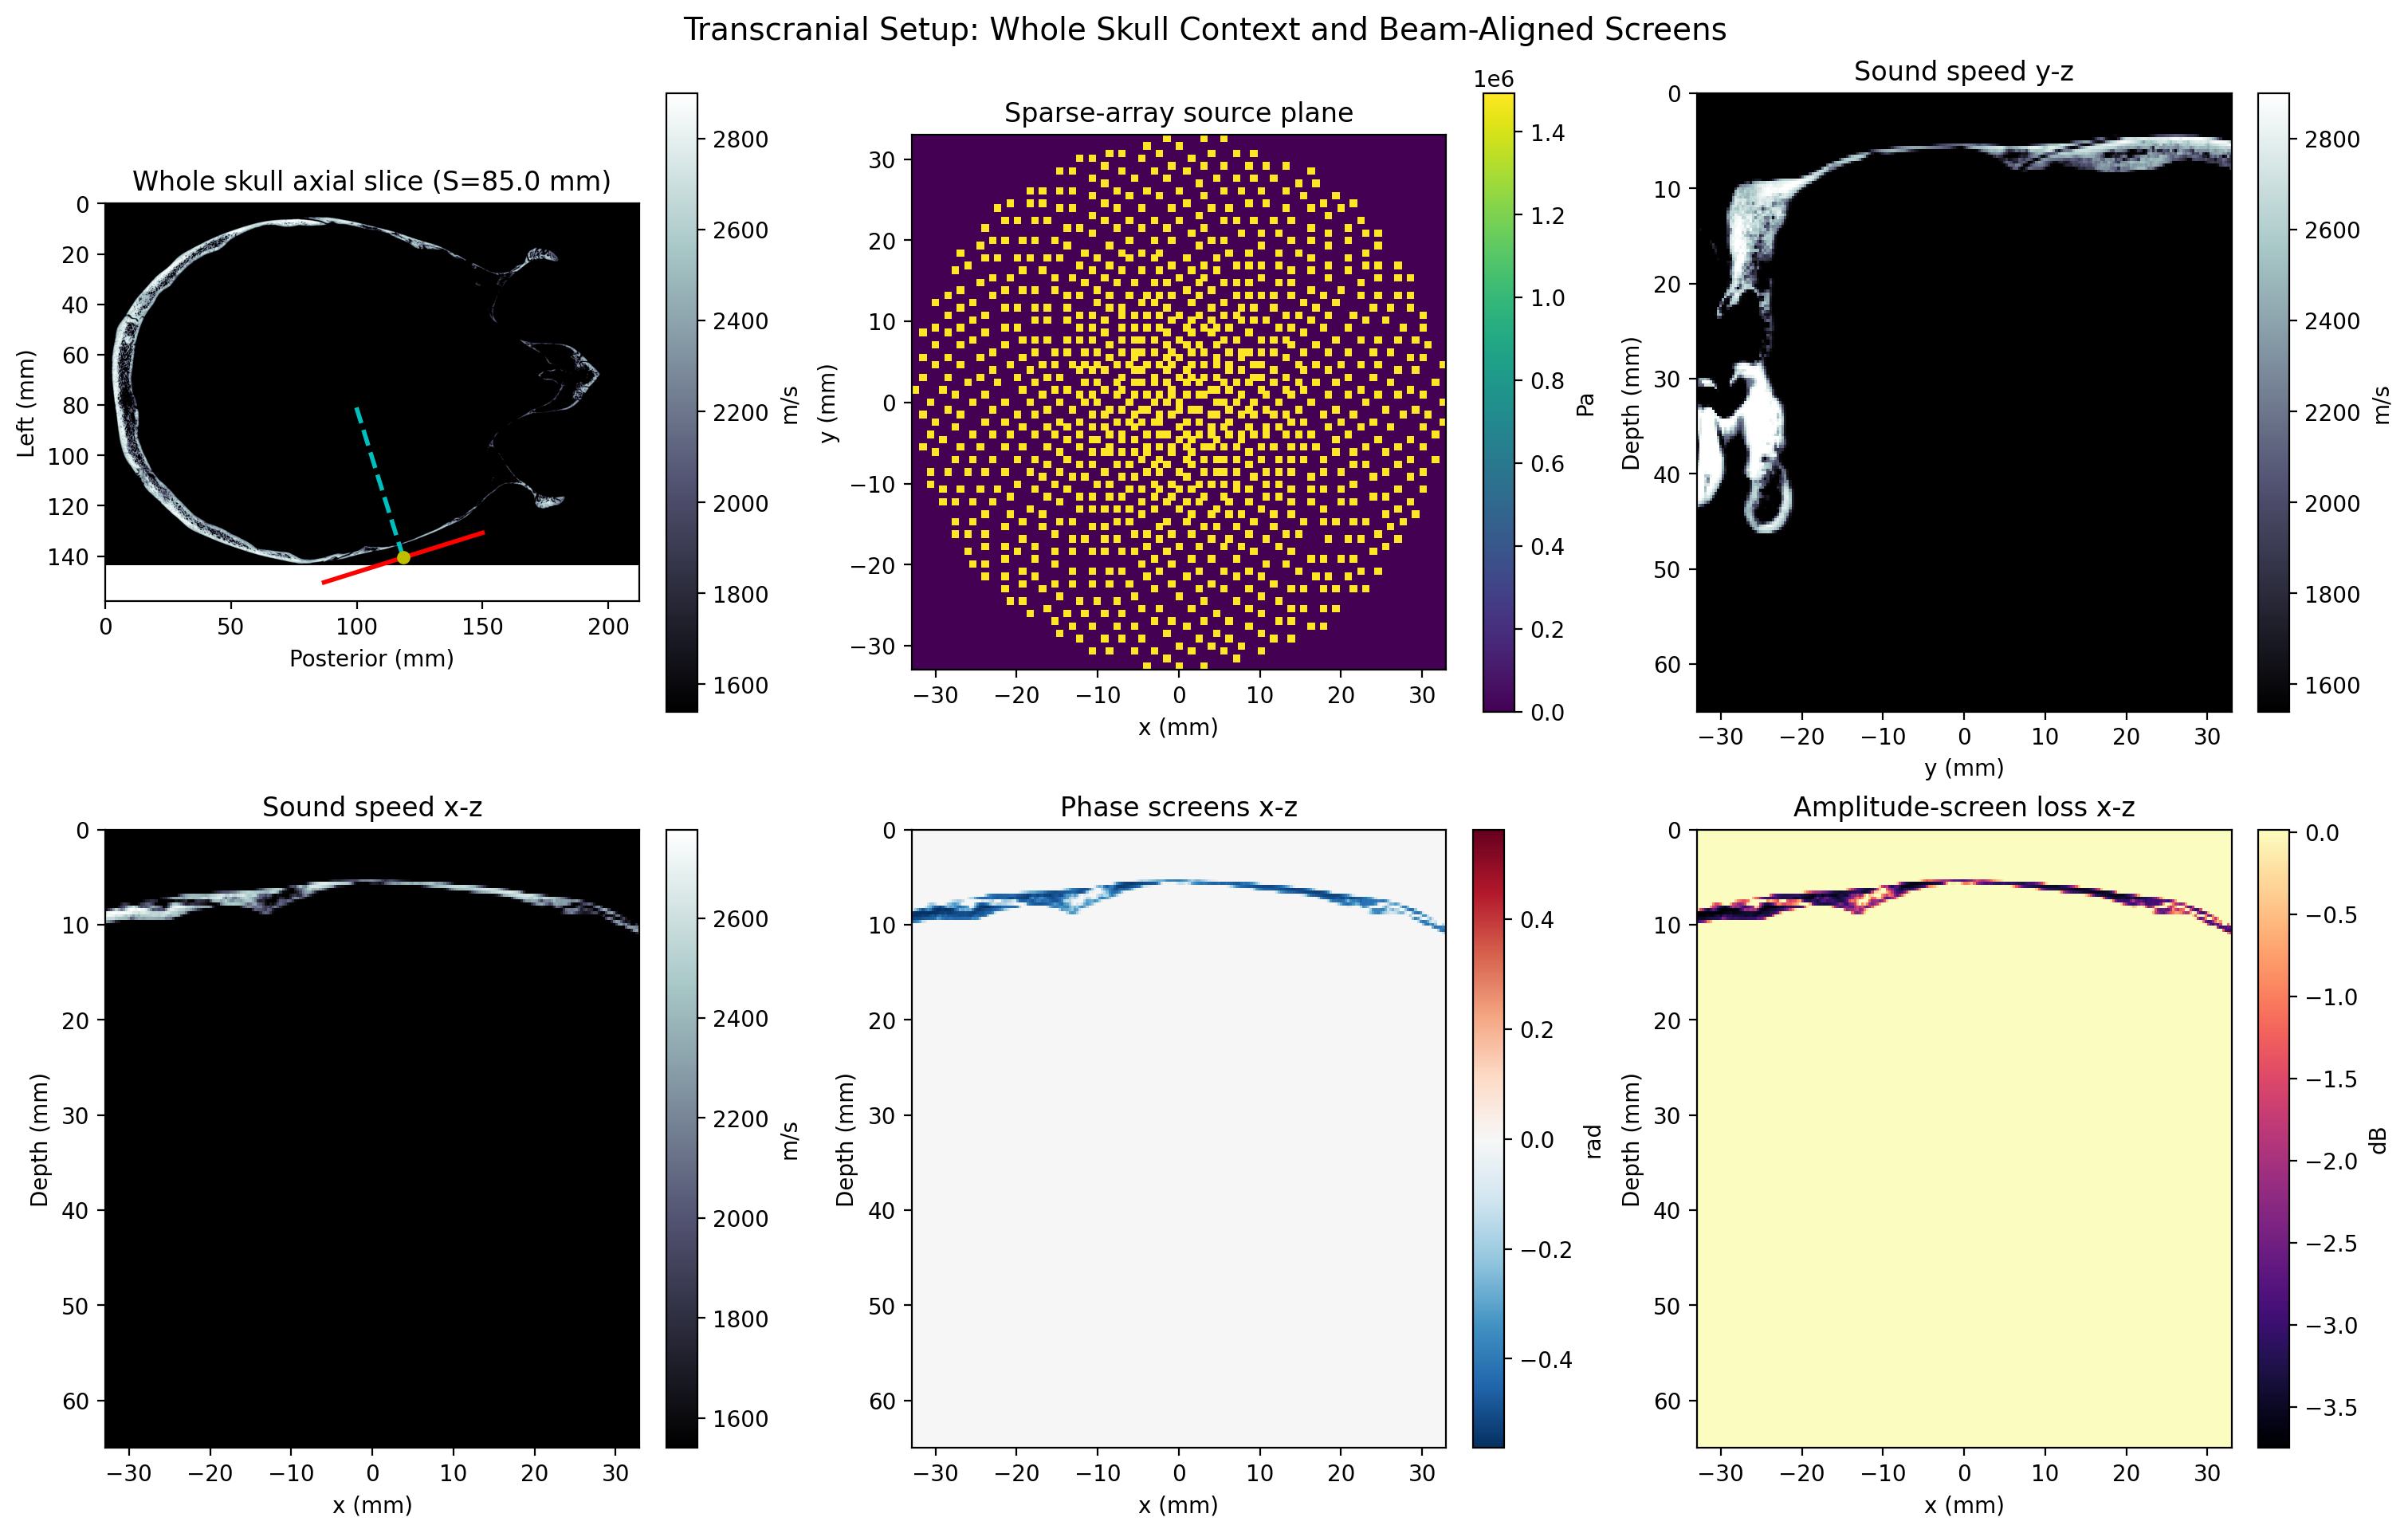
\includegraphics[width=\columnwidth]{validation_results/transcranial/setup_overview.png}
  \caption{Transcranial simulation setup.  Top left: whole-skull axial
    reference slice with beam axis overlaid.  Top center: source-plane
    pressure magnitude from the 1024-element sparse array.  Top right:
    beam-aligned sound-speed map ($y$--$z$).  Bottom left: sound-speed
    map ($x$--$z$).  Bottom center and right: stacked phase-screen and
    amplitude-screen loss maps in the $x$--$z$ plane.}
  \label{fig:transcranial_setup}
\end{figure}

\begin{figure}[htbp]
  \centering
  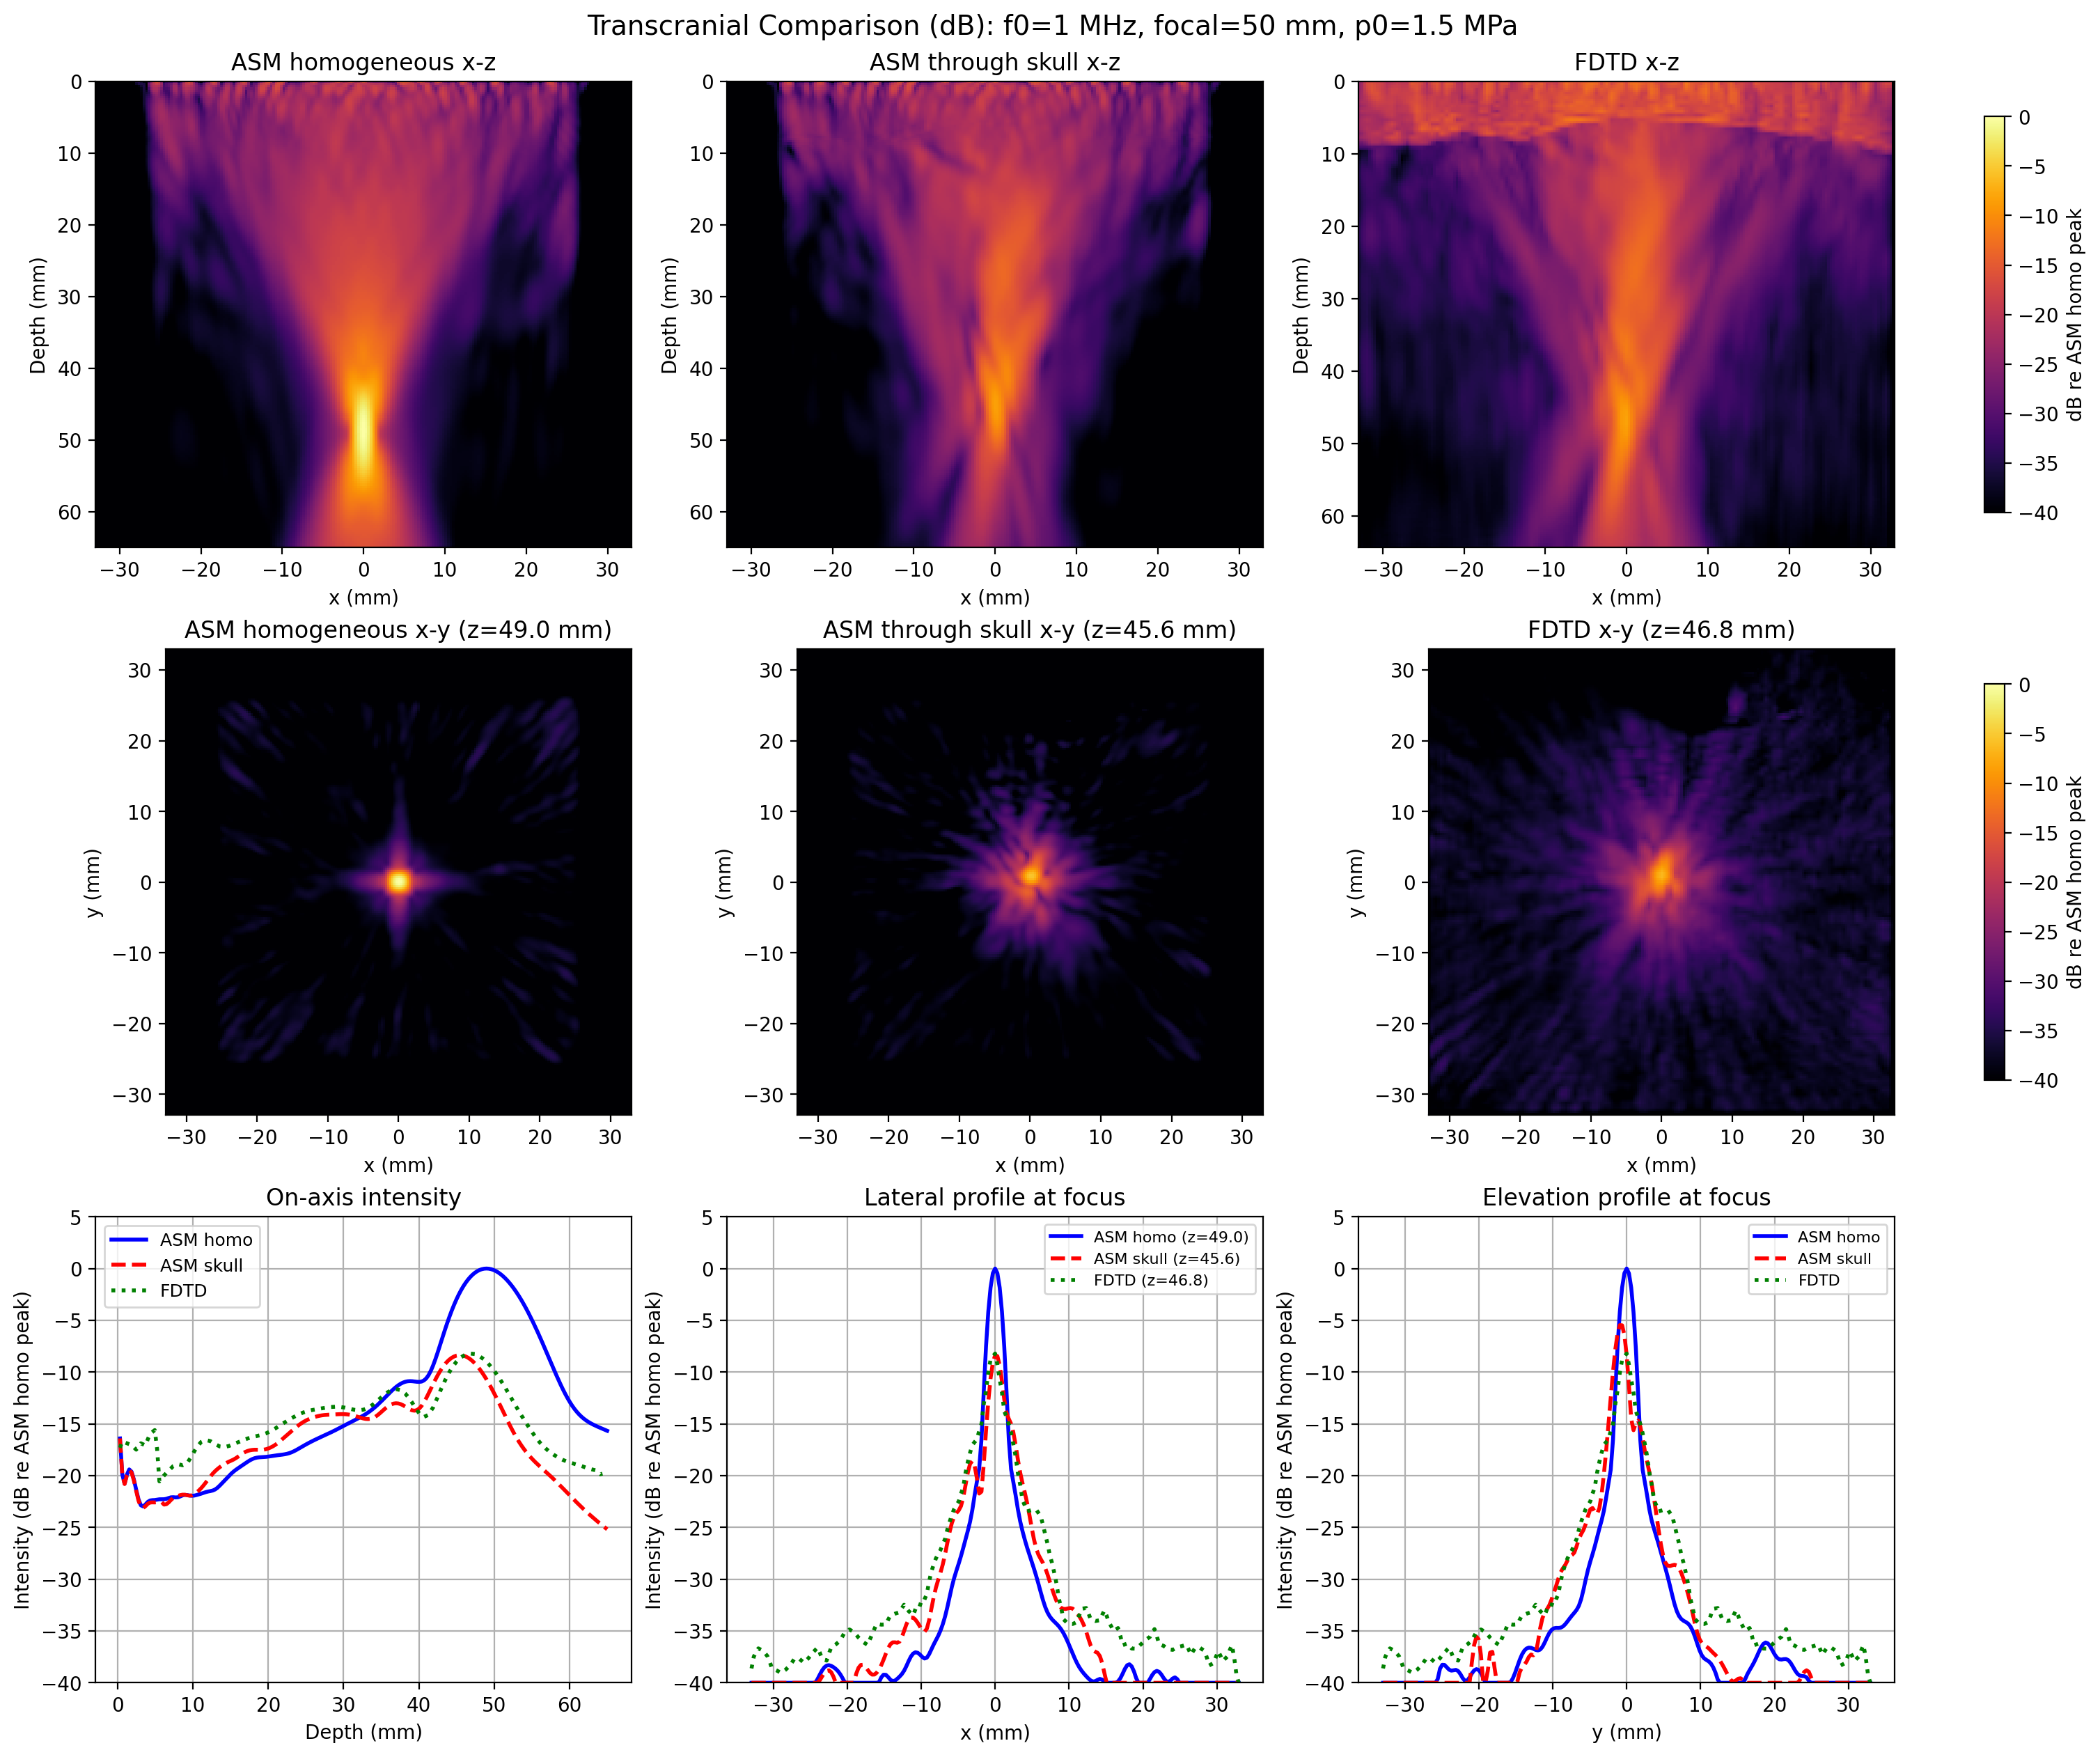
\includegraphics[width=\columnwidth]{validation_results/transcranial/transcranial_comparison.png}
  \caption{Transcranial comparison referenced to the homogeneous ASM
    field.  Top row: axial ($x$--$z$) beam profiles for ASM
    homogeneous, ASM through skull, and FDTD.  Middle row:
    corresponding focal-plane ($x$--$y$) intensity maps at each
    method's focal depth.  Bottom row: on-axis, lateral ($x$), and
    elevational ($y$) profiles in dB.  The FDTD intensity is weighted
    by its recorded temporal sampling interval before normalization so
    the dB offsets are consistent with the ASM time-integrated
    intensity.}
  \label{fig:transcranial_profiles}
\end{figure}

% ------------------------------------------------------------------
\section{Immersed bowl transducer model}
\label{sec:bowl}

\subsection{Motivation}
\label{sec:bowl:motivation}

The sparse-array validation of \cref{sec:transcranial} uses a
geometrically flat source aperture: all elements lie in a single
$z = 0$ plane, and focusing is achieved entirely through electronic
time delays.  Therapeutic transducers such as the TIPS (Therapeutic
Imaging Probe and Sonication, Philips) employ a spherical bowl
geometry with a radius of curvature $R = \SI{80}{\milli\meter}$, an
annular aperture ($r_{\mathrm{in}} = \SI{20.5}{\milli\meter}$,
$r_{\mathrm{out}} = \SI{46}{\milli\meter}$), and eight concentric
annular elements.  The bowl depth at the rim is
\begin{equation}
  d_{\mathrm{bowl}} = R - \sqrt{R^2 - r_{\mathrm{out}}^2}
  \approx \SI{14.6}{\milli\meter} \approx 9.5\lambda,
\end{equation}
which is too deep for a single-plane time-delay projection to
accurately capture the converging wavefront.

\subsection{Plane-by-plane source injection}
\label{sec:bowl:injection}

We decompose the bowl surface into thin axial slices of thickness
$\Delta z$ aligned with the propagation step.  Each slice contains the
annular ring of transducer surface lying between $z_i$ and
$z_i + \Delta z$, where $z = 0$ is the bowl apex and
$z(r) = R - \sqrt{R^2 - r^2}$ maps lateral position to bowl depth.

For a given electronic focal depth $z_f$ (which may differ from the
geometric focus at $R$), the focusing delay at each surface point
$(x, y, z_{\mathrm{bowl}})$ is computed from the distance to the
focal point:
\begin{equation}
  d(x,y) = \sqrt{x^2 + y^2 + (z_f - z_{\mathrm{bowl}})^2},
  \qquad
  \tau(x,y) = \frac{d_{\max} - d(x,y)}{c_0},
  \label{eq:bowl_delay}
\end{equation}
so that the outermost elements fire first and all wavefronts converge
at $z_f$.  For an annular phased array, the per-pixel delays are
averaged within each element to produce per-element delays, matching
the hardware constraint.

During propagation, the solver starts from the apex slice
($z = 0$) and marches forward.  As it crosses each slice depth $z_i$,
the corresponding source field is \emph{added} to the propagating
wavefield:
\begin{equation}
  p(\mathbf{x}, t)\big|_{z = z_i^+}
  = p(\mathbf{x}, t)\big|_{z = z_i^-}
  + s_i(\mathbf{x}, t),
\end{equation}
where $s_i$ is the time-delayed pulse restricted to the annular ring
in the $i$-th slice, with its delay corrected by $-z_i/c_0$ to account
for the propagation distance already traversed from the apex.  This
injection is implemented identically to the phase-screen application:
a simple conditional addition at the appropriate $z$ coordinate within
the main propagation loop.

\subsection{FDTD comparison}
\label{sec:bowl:results}

To validate the plane-by-plane model, we compare the ASM prediction
against a 3-D FDTD simulation in water.  The TIPS bowl is focused
electronically at \SI{50}{\milli\meter} (inside the geometric focus at
$R = \SI{80}{\milli\meter}$) using a \SI{1}{\mega\hertz}, 3-cycle
Gaussian-windowed pulse at $p_0 = \SI{400}{\kilo\pascal}$.

The FDTD reference uses the volumetric bowl source (3 voxel layers
along the surface normal) solved on a $623 \times 873 \times 873$ grid
at $\Delta x = \SI{0.128}{\milli\meter}$ ($\lambda/12$) with 6234 time
steps.  The ASM uses $\Delta x = \lambda/5$ with a
$365 \times 365 \times 425$ grid and 260 propagation steps
($\Delta z = \Delta x$).

Figure~\ref{fig:tips_setup} shows the TIPS transducer geometry: the
bowl cross-section with element boundaries and focal lines, the
plane-by-plane source slices spanning the
\SI{14.6}{\milli\meter} bowl depth, the 8-element annular aperture,
and the per-element focusing delays.

Figure~\ref{fig:tips_comparison} compares the plane-by-plane ASM
against the FDTD reference.  Each method is normalized to its own
peak intensity so the beam shapes can be compared directly.
The ASM focuses at $z = \SI{52.7}{\milli\meter}$, within 2.3\% of
the FDTD focal depth at \SI{53.9}{\milli\meter}.
The on-axis, lateral, and elevational beam profiles match well in
shape. The remaining differences are concentrated in the pre-focal
near-field where the annular aperture geometry produces
resolution-dependent interference fringes.
The FDTD drives the bowl surface with three voxel layers extruded
along the surface normal, whereas the ASM injects a single layer per
$z$-slice.  To match the FDTD source coupling, the ASM source amplitude is scaled
by a calibration factor of 1.31.  This factor accounts for the
coherent array factor of the three-layer volumetric source at the FDTD
grid spacing ($k \Delta x \approx 0.79$\,rad, CFL $= 0.2$) and is
specific to this FDTD configuration and would need to be recalibrated
for a different number of layers or grid resolution.  After
calibration, both methods produce a focal peak pressure of
\SI{13.8}{\mega\pascal}.

The ASM requires substantially less memory than the FDTD.  The FDTD
solver allocates the full 3-D volume
($623 \times 873 \times 873 \approx \SI{475}{M}$ grid points) for
approximately eight field arrays (pressure, velocity components,
material maps), totaling roughly \SI{15}{\giga\byte}.  The ASM
stores only the current 2-D-plus-time field
($365 \times 365 \times 425 \approx \SI{57}{M}$ points) together with
precomputed frequency-domain operators of the same shape, for a total
of approximately \SI{1.6}{\giga\byte}, a factor of nine reduction.
For the present benchmark the FDTD completes in \SI{1477}{\second}
(multi-GPU) while the ASM requires \SI{516}{\second} (single GPU),
a $2.9\times$ speed-up despite using only one GPU.  The ASM wall time
is dominated by its 260 sequential FFT-based propagation steps and
could be reduced further with a coarser axial step.

\begin{figure}[htbp]
  \centering
  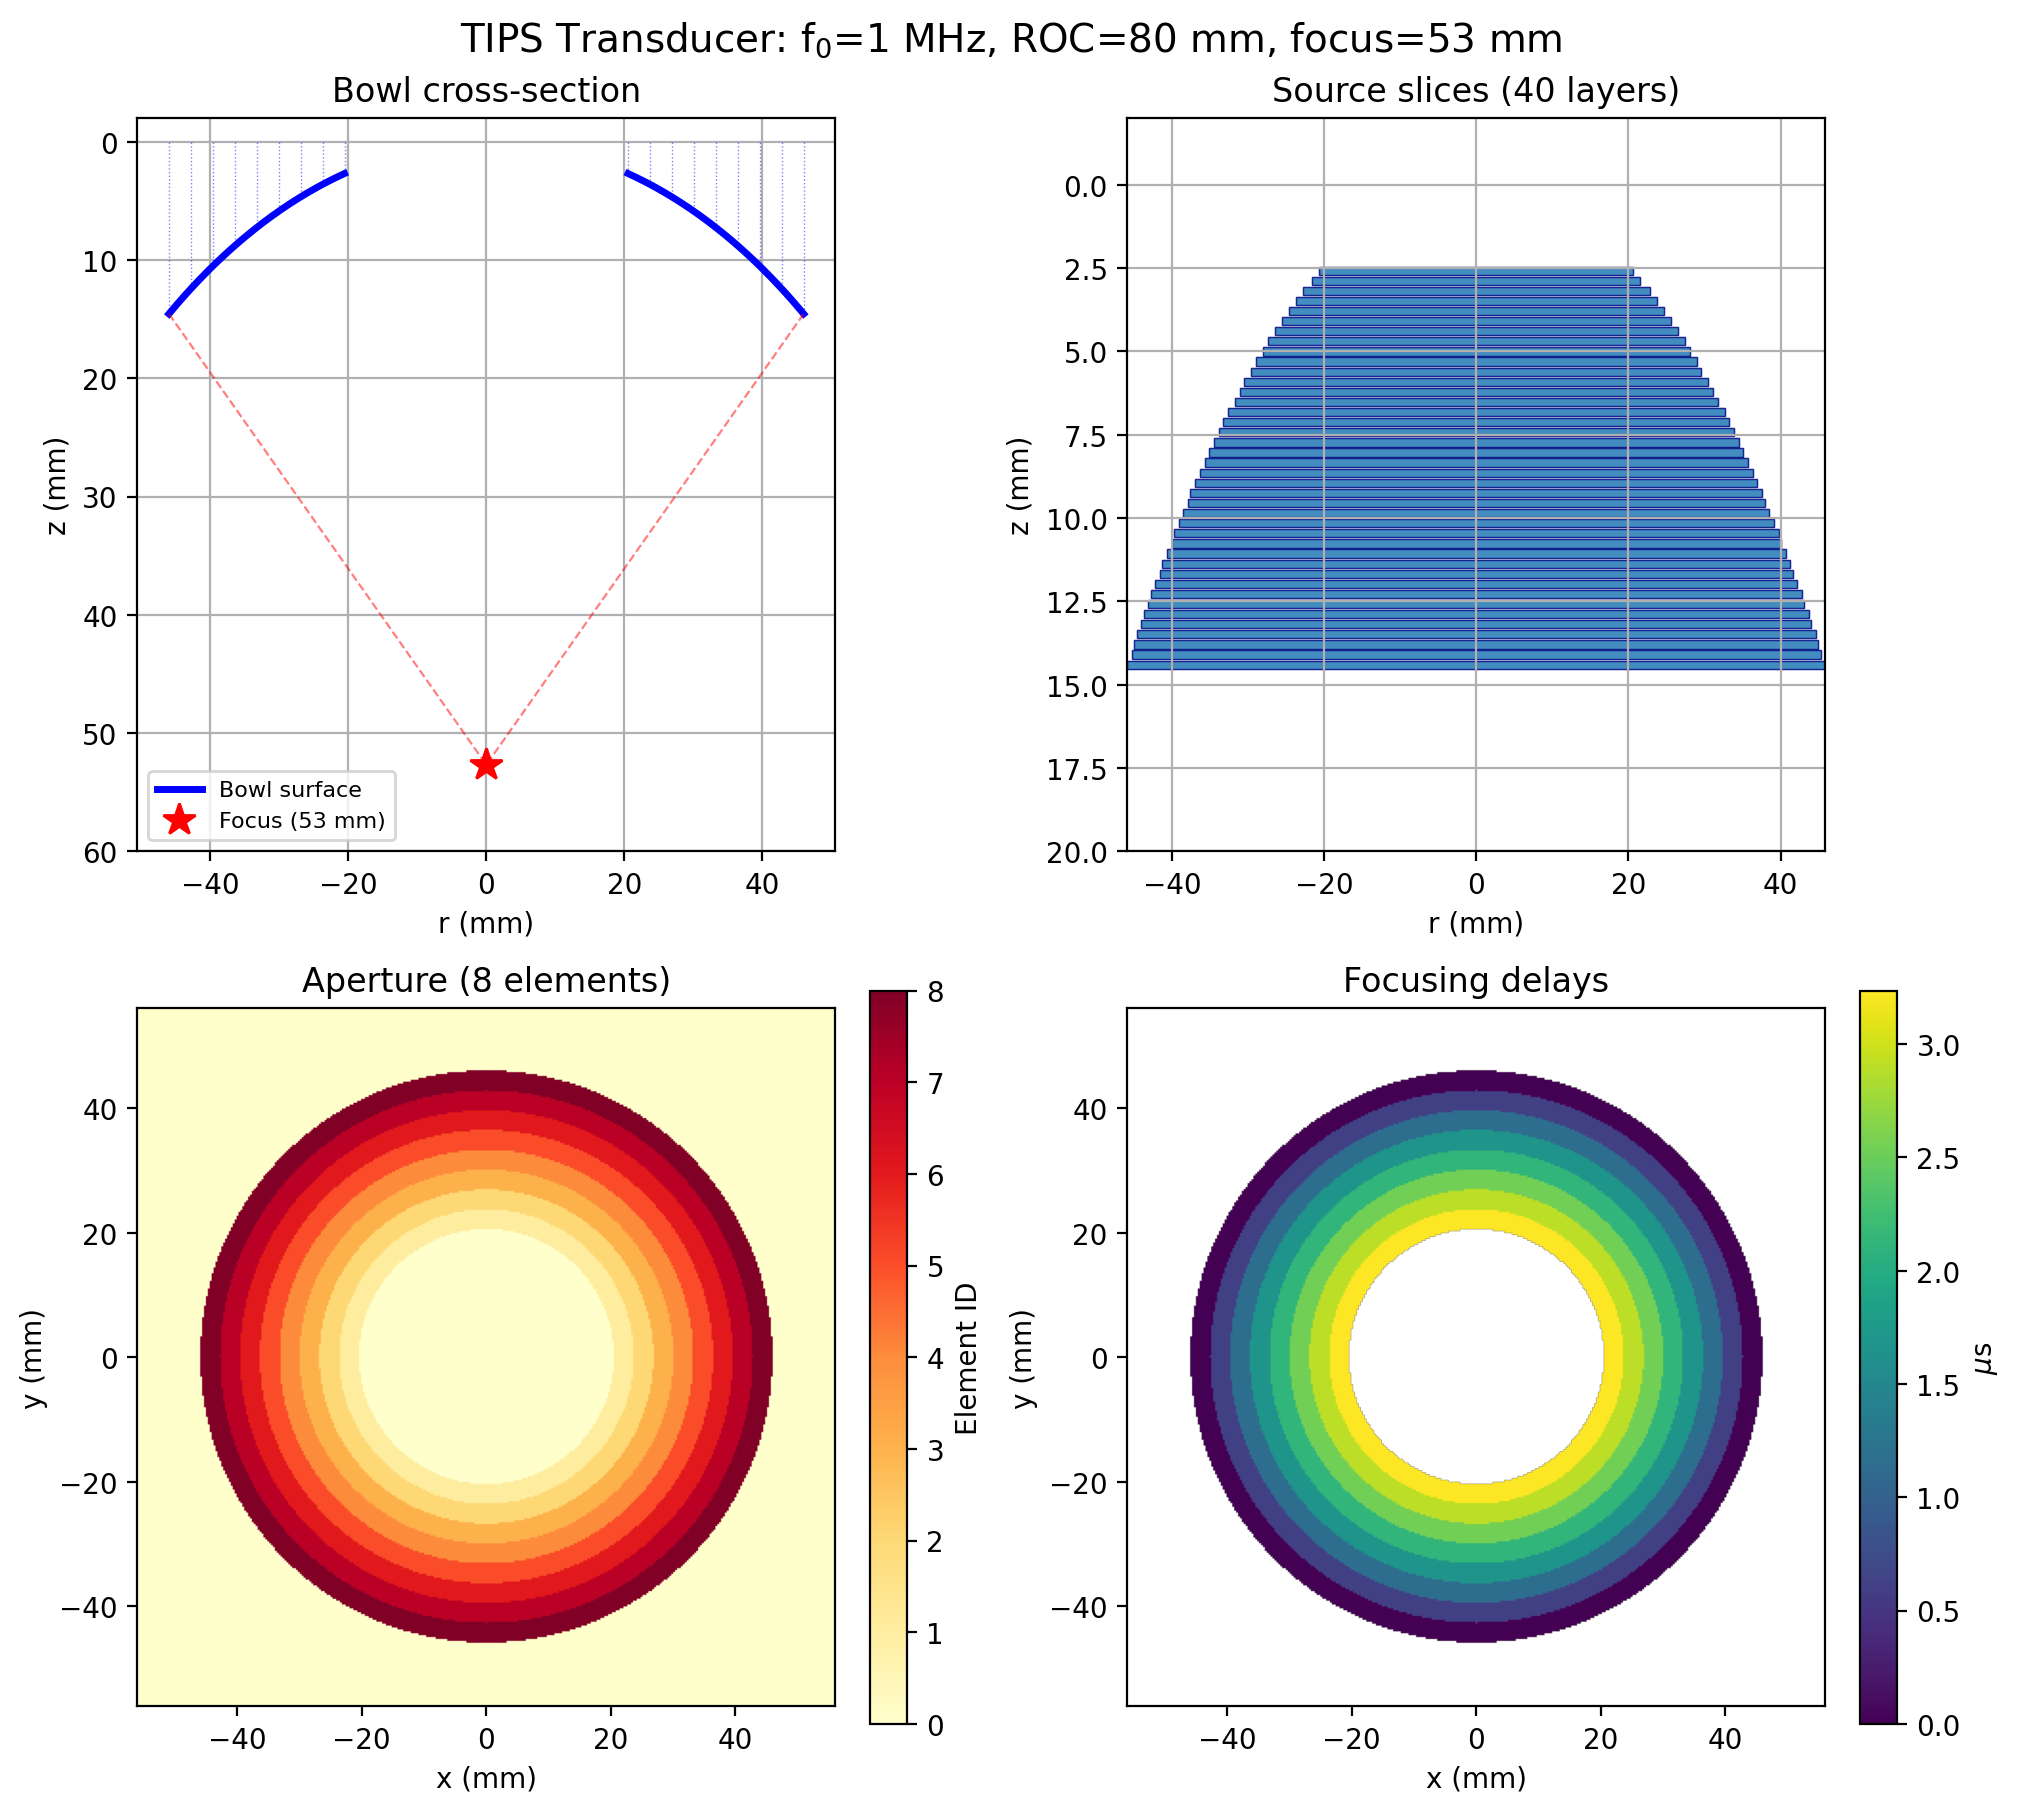
\includegraphics[width=\columnwidth]{validation_results/bowl/tips_setup.png}
  \caption{TIPS bowl transducer setup.  Top left: bowl cross-section
    ($R = \SI{80}{\milli\meter}$) with element boundaries and focal
    lines.  Top right: plane-by-plane source slices spanning the
    \SI{14.6}{\milli\meter} bowl depth.  Bottom left: 8-element
    annular aperture.  Bottom right: per-element focusing delays.}
  \label{fig:tips_setup}
\end{figure}

\begin{figure}[htbp]
  \centering
  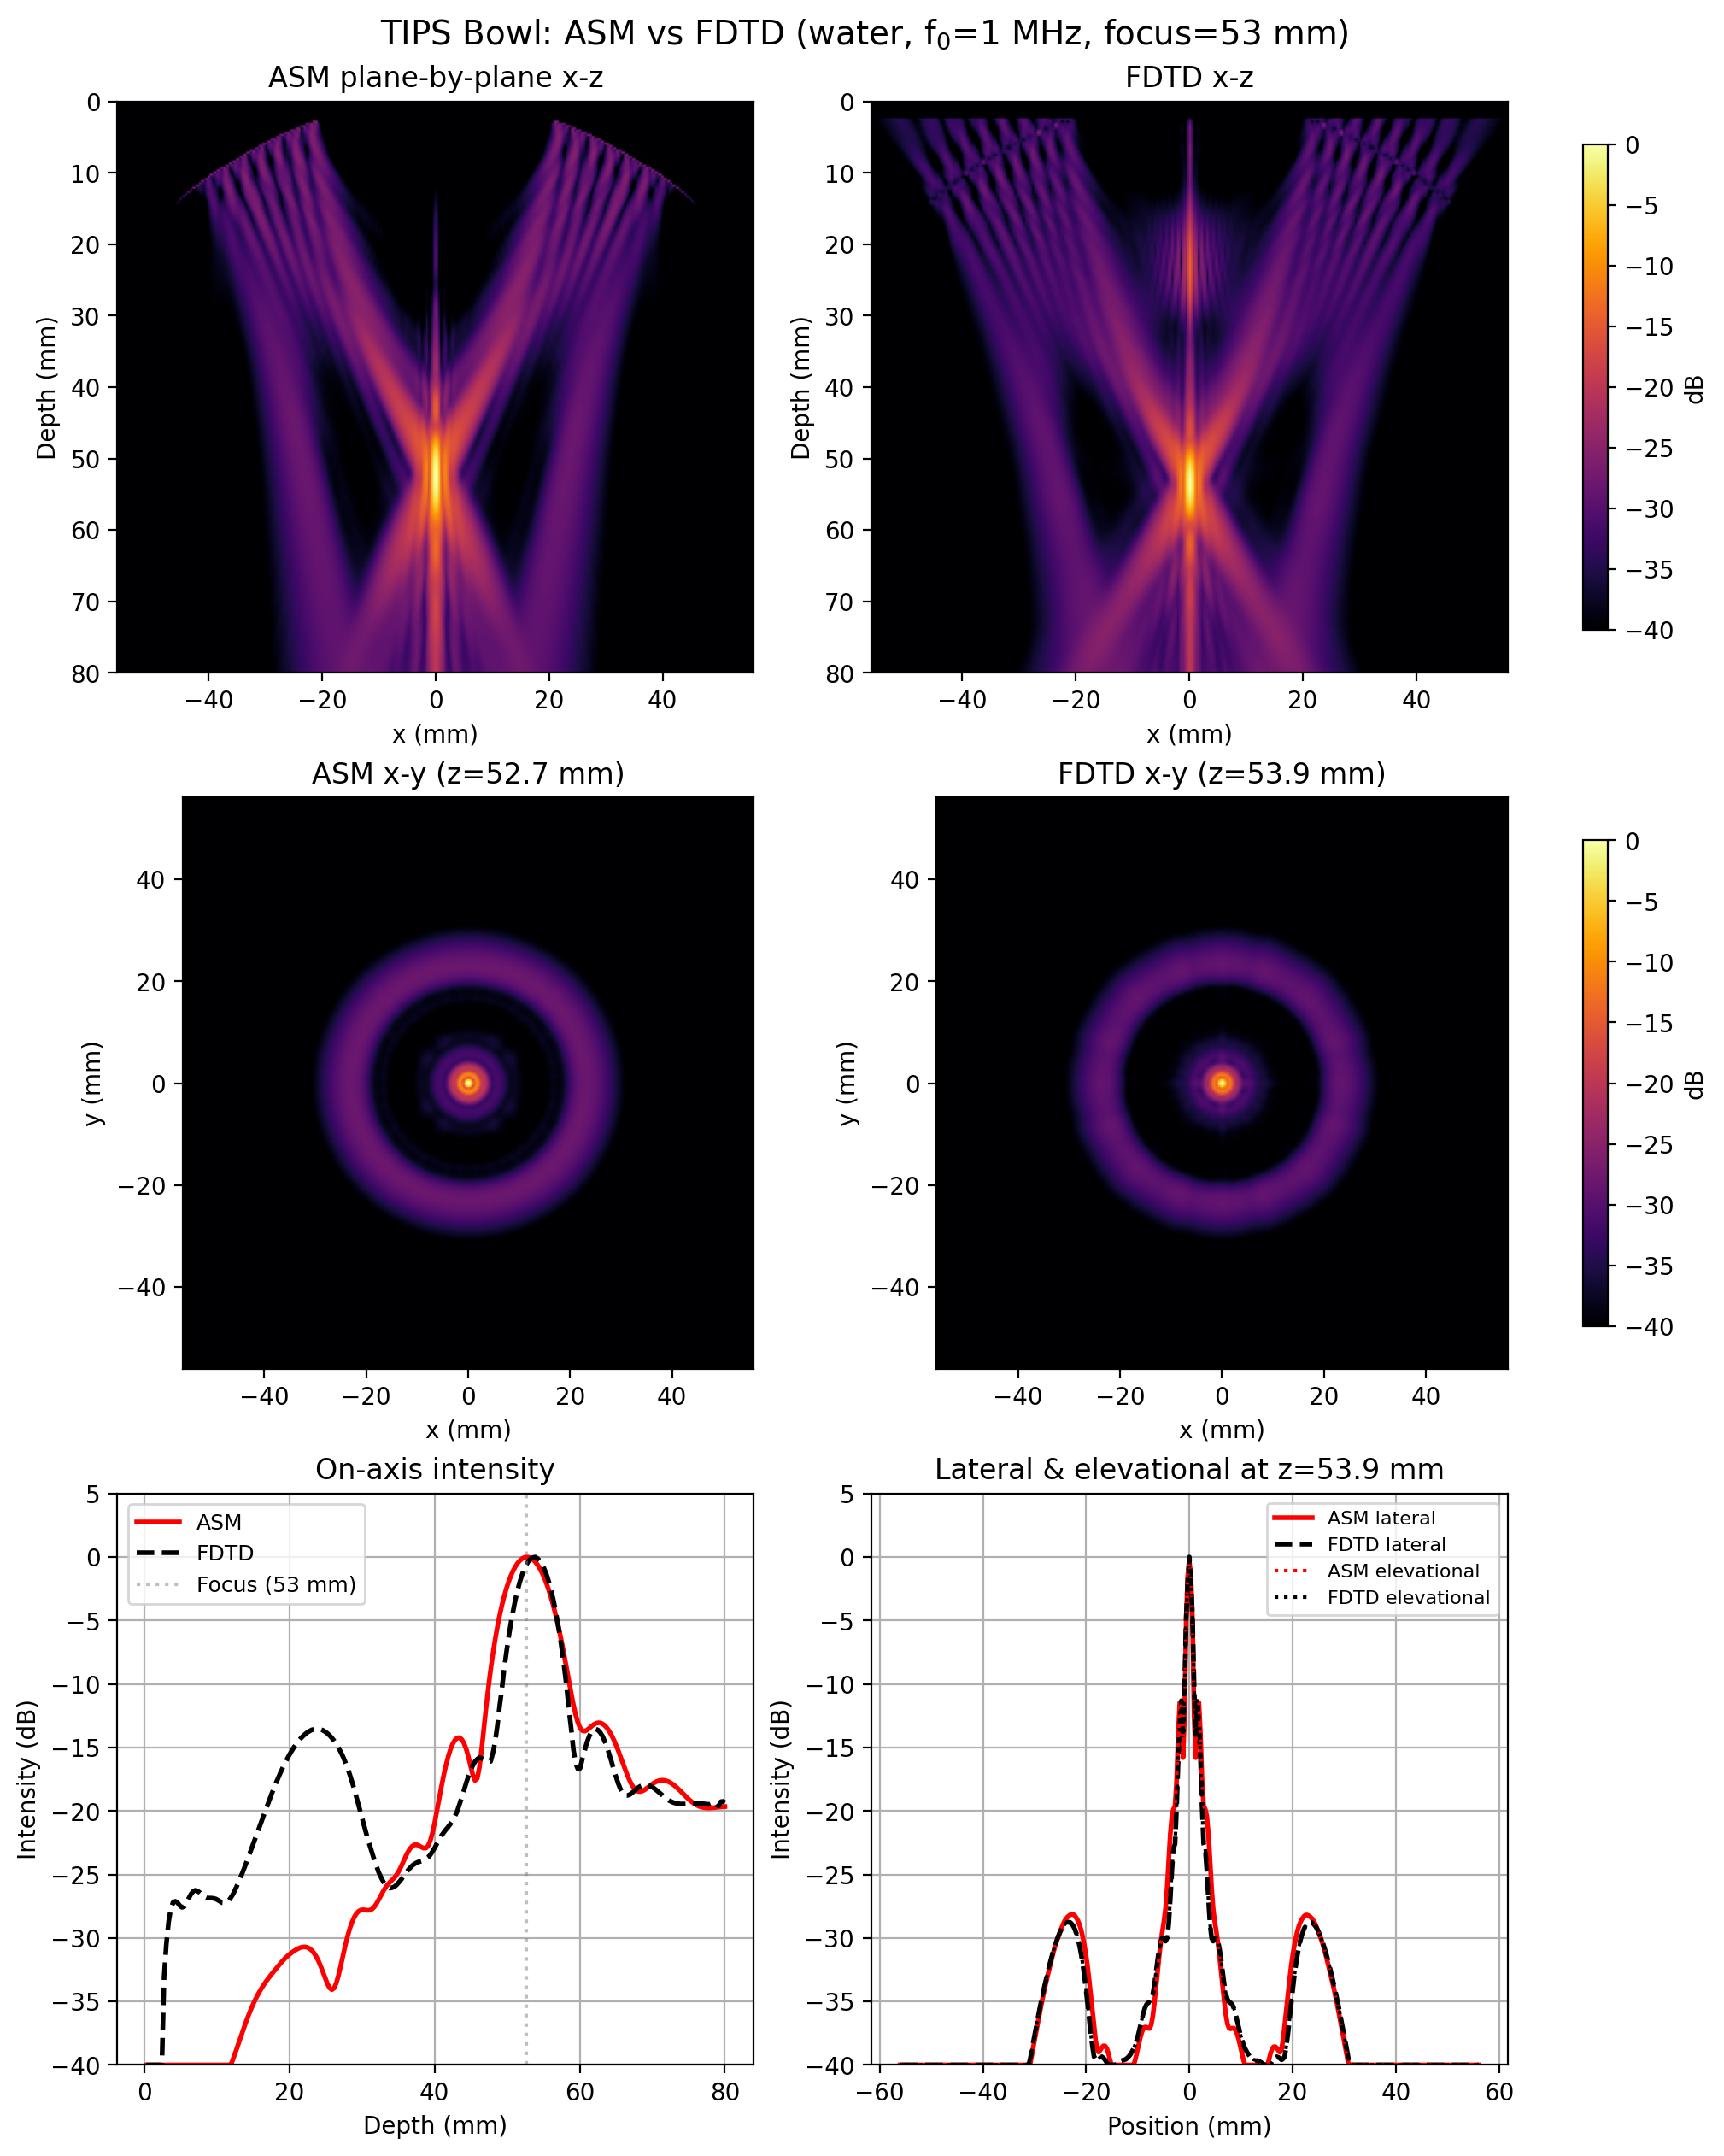
\includegraphics[width=\columnwidth]{validation_results/bowl/tips_comparison.png}
  \caption{TIPS bowl comparison: ASM plane-by-plane vs FDTD in water.
    Top row: axial ($x$--$z$) beam profiles.  Middle row: focal-plane
    ($x$--$y$) intensity maps at each method's focal depth.  Bottom
    left: on-axis intensity.  Bottom right: lateral and elevational
    profiles at the FDTD focal depth.  Each method is normalized to
    its own peak so the beam shapes can be compared directly.  The ASM
    focal depth (\SI{52.7}{\milli\meter}) matches the FDTD
    (\SI{53.9}{\milli\meter}) to within 2.3\%.}
  \label{fig:tips_comparison}
\end{figure}

% ------------------------------------------------------------------
\section{Discussion}
\label{sec:discussion}

The results establish that the angular spectrum method, extended with
phase-and-amplitude screens and plane-by-plane source injection, can
reproduce FDTD-quality focal fields at a fraction of the computational
cost for both transcranial and therapeutic ultrasound configurations.

The diffraction benchmarks confirm that the propagator correctly
handles both unfocused and geometrically focused sources, matching
analytical Rayleigh--Fresnel and Airy solutions with RMS errors of
0.086 (on-axis) and 0.002 (focal plane).  The Strang+KT splitting
achieves second-order convergence (rate $\approx 2$) in the strongly
nonlinear regime, compared with first-order for the sequential and
Rusanov-based schemes.  The KT flux resolves shocks more sharply than
Rusanov ($L^2$ error 0.036 vs.\ 0.044), and the adaptive CFL
sub-cycling guarantees stability at all step sizes while preserving
accuracy.

The three boundary improvements act cumulatively, reducing the
periodic-FFT reflection ratio by $2.4\times$ without distorting the
interior field.  The frequency-weighted damping preferentially targets
low-frequency components that see fewer wavelengths in the boundary
layer, while the Engquist--Majda super-absorbing correction selectively
removes incoming wave energy.

In the transcranial benchmark, the phase-and-amplitude-screen ASM
matches the FDTD focal-plane intensity with 1.1\% RMS difference and
predicts a through-skull insertion loss of \SI{5.4}{\deci\bel},
consistent with measured values of
\SIrange{5}{10}{\deci\bel}~\cite{pinton2012}.  The focal depth
differs by only 2.6\% from the FDTD reference.  The TIPS bowl
validation extends this agreement to a curved-source geometry: the
plane-by-plane ASM matches the FDTD focal depth to within 2.3\% while
requiring $9\times$ less memory and $2.9\times$ less wall time.

Several limitations should be noted.  The ASM is a forward-only
propagator: the phase-and-amplitude-screen model captures the dominant
wavefront aberration and insertion loss but neglects reflection, mode
conversion, and multiple scattering at acoustic interfaces.  The
remaining discrepancy with FDTD in the transcranial benchmark is
concentrated in the pre-focal region and near the skull surface where
these backward-propagating effects are strongest.  For the bowl
transducer, the FDTD's multi-layer volumetric source couples
differently from the ASM's single-layer planar injection, requiring an
empirical amplitude calibration factor (here 1.31) that depends on the
FDTD grid spacing and number of source layers.  The super-absorbing
boundary uses a first-order Engquist--Majda decomposition, which is
exact only for normally-incident waves. A higher-order formulation
\cite{higdon1986} could improve performance for wide-angle beams.
Finally, although the Strang+KT splitting achieves second-order
convergence when the nonlinear operator is tested in isolation, the
full coupled solver includes additional error contributions from
diffraction, transverse discretization, and the split-step composition
of three operators, so the observed global convergence rate remains
below two.

% ------------------------------------------------------------------
\section{Conclusion}
\label{sec:conclusion}

Two extensions to the angular spectrum method have been presented that
address practical barriers to its use in transcranial and therapeutic
ultrasound.  Phase-and-amplitude screens derived from CT data
incorporate skull-induced aberration and frequency-dependent insertion
loss into the FFT-based propagator, matching an FDTD reference to
1.1\% RMS in focal-plane intensity and predicting a through-skull
insertion loss of \SI{5.4}{\deci\bel}, consistent with measured
values.  Plane-by-plane source injection enables accurate modeling of
spherical-bowl transducers whose curvature depth exceeds the
wavelength. For a clinical TIPS annular array, the method matches the
FDTD focal depth to within 2.3\% while requiring $9\times$ less
memory and $2.9\times$ less wall time.

On the numerical side, the second-order Kurganov--Tadmor flux with
Strang splitting achieves rate-2 convergence and, with adaptive CFL
sub-cycling, remains stable at all tested step sizes.  Three
absorbing-boundary improvements reduce periodic-FFT reflections by
$2.4\times$ without distorting the interior field.  The intensity-loss
tracking provides a spatially resolved absorbed-energy map that
accounts for the full harmonic content of the nonlinear wave, suitable
for radiation-force and thermal dose calculations.

Together, these developments extend the practical reach of the angular
spectrum method from homogeneous free-field propagation to
heterogeneous transcranial paths and immersed curved-source
geometries, at computational costs that are compatible with treatment
planning and real-time aberration correction workflows.

\section*{Acknowledgments}

This work was supported by the National Institutes of Health under
grants R01EB029419 and R01EB036295.

% ------------------------------------------------------------------
The source code and all validation scripts needed to reproduce the
figures in this paper are available at
\url{https://github.com/gfpinton/angularspectrum_python}.

\begin{thebibliography}{20}

\bibitem{christopher1991}
P.~T. Christopher and K.~J. Parker,
``New approaches to nonlinear diffractive field propagation,''
\textit{J.\ Acoust.\ Soc.\ Am.}, vol.~90, no.~1, pp.~488--499, 1991.

\bibitem{dagrau2011}
F.~Dagrau, M.~R\'{e}nier, R.~Marchiano, and F.~Coulouvrat,
``Acoustic shock wave propagation in a heterogeneous medium: a
numerical simulation beyond the parabolic approximation,''
\textit{J.\ Acoust.\ Soc.\ Am.}, vol.~130, no.~1, pp.~20--32, 2011.

\bibitem{du1985}
G.~Du and M.~A. Breazeale,
``The ultrasonic field of a Gaussian transducer,''
\textit{J.\ Acoust.\ Soc.\ Am.}, vol.~78, no.~6, pp.~2083--2086, 1985.

\bibitem{engquist1977}
B.~Engquist and A.~Majda,
``Absorbing boundary conditions for the numerical simulation of waves,''
\textit{Math.\ Comp.}, vol.~31, no.~139, pp.~629--651, 1977.

\bibitem{giammarinaro2016}
B.~Giammarinaro, F.~Coulouvrat, and G.~Pinton,
``Numerical simulation of focused shock shear waves in soft solids and
a two-dimensional nonlinear homogeneous model of the brain,''
\textit{J.\ Biomech.\ Eng.}, vol.~138, no.~4, art.~041003, 2016.

\bibitem{gottlieb2001}
S.~Gottlieb, C.-W. Shu, and E.~Tadmor,
``Strong stability-preserving high-order time discretization methods,''
\textit{SIAM Rev.}, vol.~43, no.~1, pp.~89--112, 2001.

\bibitem{halle_skull}
``Halle skull microCT dataset,'' Zenodo, 2022,
doi: 10.5281/zenodo.6956658.

\bibitem{higdon1986}
R.~L. Higdon,
``Absorbing boundary conditions for difference approximations to the
multi-dimensional wave equation,''
\textit{Math.\ Comp.}, vol.~47, no.~176, pp.~437--459, 1986.

\bibitem{jax2018}
J.~Bradbury \textit{et~al.},
``JAX: composable transformations of Python+NumPy programs,''
2018. [Online]. Available: \url{http://github.com/google/jax}

\bibitem{kinsler2000}
L.~E. Kinsler, A.~R. Frey, A.~B. Coppens, and J.~V. Sanders,
\textit{Fundamentals of Acoustics}, 4th ed.\ New York: Wiley, 2000.

\bibitem{luo2020}
H.~Luo, J.~Kusunose, G.~Pinton, C.~F. Caskey, and W.~A. Grissom,
``Rapid quantitative imaging of high intensity ultrasonic pressure
fields,''
\textit{J.\ Acoust.\ Soc.\ Am.}, vol.~148, no.~2, pp.~660--668, 2020.

\bibitem{leveque2002}
R.~J. LeVeque,
\textit{Finite Volume Methods for Hyperbolic Problems}.
Cambridge: Cambridge Univ.\ Press, 2002.

\bibitem{kurganov2000}
A.~Kurganov and E.~Tadmor,
``New high-resolution central schemes for nonlinear conservation laws
and convection--diffusion equations,''
\textit{J.\ Comput.\ Phys.}, vol.~160, no.~1, pp.~241--282, 2000.

\bibitem{martin1988}
J.~M. Martin and S.~M. Flatt\'{e},
``Intensity images and statistics from numerical simulation of wave
propagation in 3-D random media,''
\textit{Appl.\ Opt.}, vol.~27, no.~11, pp.~2111--2126, 1988.

\bibitem{pinton2012}
G.~F. Pinton, J.-F. Aubry, E.~Bossy, M.~Muller, M.~Pernot, and M.~Tanter,
``Attenuation, scattering, and absorption of ultrasound in the skull bone,''
\textit{Med.\ Phys.}, vol.~39, no.~1, pp.~299--307, 2012.

\bibitem{nyborg1981}
W.~L. Nyborg,
``Heat generation by ultrasound in a relaxing medium,''
\textit{J.\ Acoust.\ Soc.\ Am.}, vol.~70, no.~2, pp.~310--312, 1981.

\bibitem{pinton2010}
G.~F. Pinton, F.~Coulouvrat, J.-L. Gennisson, and M.~Tanter,
``Nonlinear reflection of shock shear waves in soft elastic media,''
\textit{J.\ Acoust.\ Soc.\ Am.}, vol.~127, no.~2, pp.~683--691, 2010.

\bibitem{pinton2014}
G.~F. Pinton,
``Numerical methods for nonlinear wave propagation in ultrasound,''
Ph.D.\ dissertation, Dept.\ Biomed.\ Eng., Duke Univ., Durham, NC, 2007.

\bibitem{pinton2009}
G.~F. Pinton, J.~Dahl, S.~Rosenzweig, and G.~E. Trahey,
``A heterogeneous nonlinear attenuating full-wave model of ultrasound,''
\textit{IEEE Trans.\ Ultrason., Ferroelect., Freq.\ Control},
vol.~56, no.~3, pp.~474--488, 2009.

\bibitem{rusanov1962}
V.~V. Rusanov,
``Calculation of interaction of non-steady shock waves with obstacles,''
\textit{J.\ Comput.\ Math.\ Phys.\ USSR}, vol.~1, pp.~267--279, 1962.

\bibitem{szabo1995}
T.~L. Szabo,
``Causal theories and data for acoustic attenuation obeying a
frequency power law,''
\textit{J.\ Acoust.\ Soc.\ Am.}, vol.~97, no.~1, pp.~14--24, 1995.

\bibitem{strang1968}
G.~Strang,
``On the construction and comparison of difference schemes,''
\textit{SIAM J.\ Numer.\ Anal.}, vol.~5, no.~3, pp.~506--517, 1968.

\bibitem{vanleer1979}
B.~van~Leer,
``Towards the ultimate conservative difference scheme.~V.~A
second-order sequel to Godunov's method,''
\textit{J.\ Comput.\ Phys.}, vol.~32, no.~1, pp.~101--136, 1979.

\bibitem{treeby2012}
B.~E. Treeby, J.~Jaros, A.~P. Rendell, and B.~T. Cox,
``Modeling nonlinear ultrasound propagation in heterogeneous media
with power law absorption using a $k$-space pseudospectral method,''
\textit{J.\ Acoust.\ Soc.\ Am.}, vol.~131, no.~6, pp.~4324--4336, 2012.

\bibitem{yoshida1990}
H.~Yoshida,
``Construction of higher order symplectic integrators,''
\textit{Phys.\ Lett.\ A}, vol.~150, no.~5--7, pp.~262--268, 1990.

\bibitem{waters2005}
K.~R. Waters, J.~Mobley, and J.~G. Miller,
``Causality-imposed (Kramers--Kronig) relationships between
attenuation and dispersion,''
\textit{IEEE Trans.\ Ultrason., Ferroelect., Freq.\ Control},
vol.~52, no.~5, pp.~822--833, 2005.

\bibitem{wendland1995}
H.~Wendland,
``Piecewise polynomial, positive definite and compactly supported
radial functions of minimal degree,''
\textit{Adv.\ Comput.\ Math.}, vol.~4, no.~1, pp.~389--396, 1995.

\bibitem{zemp2010}
R.~J. Zemp,
``Modeling nonlinear ultrasound propagation in tissue from array
transducers,''
\textit{J.\ Acoust.\ Soc.\ Am.}, vol.~127, no.~4, pp.~2484--2494, 2010.

\end{thebibliography}

\end{document}
